\documentclass[a4paper]{article}

%% Language and font encodings
\usepackage[english]{babel}
\usepackage[utf8x]{inputenc}
\usepackage[T1]{fontenc}
\usepackage{graphicx}
\usepackage{wrapfig}
\usepackage{lscape}
\usepackage{rotating}
\usepackage{epstopdf}
%% Sets page size and margins
\usepackage[a4paper,top=3cm,bottom=2cm,left=3cm,right=3cm,marginparwidth=1.75cm]{geometry}

%% Useful packages
\usepackage{amsmath}
\usepackage{graphicx}
\usepackage[colorinlistoftodos]{todonotes}
\usepackage[colorlinks=true, allcolors=black]{hyperref}
\usepackage{amssymb}
\usepackage{graphicx}
\usepackage{subcaption}
\usepackage{wrapfig}
\usepackage{float}
\usepackage{titlesec}
\setcounter{secnumdepth}{5}
\usepackage{listings}
\usepackage{color}
 
\definecolor{codegreen}{rgb}{0,0.6,0}
\definecolor{codegray}{rgb}{0.5,0.5,0.5}
\definecolor{codepurple}{rgb}{0.58,0,0.82}
\definecolor{backcolour}{rgb}{0.95,0.95,0.92}

\lstset{
	tabsize=2,
	%commentstyle=\color{mygreen},
	numbers=left,
	numbersep=5pt,     
	stepnumber=2, 
	frame=single,
	basicstyle = \small,
	backgroundcolor=\color{backcolour},   
	commentstyle=\color{codegreen},
	basicstyle=\small,
	breaklines=true
}

\usepackage{listings}

\usepackage{todonotes}
%\newcommand\todo[1]{\textcolor{red}{#1}}

\begin{document}
\begin{titlepage} % Suppresses displaying the page number on the title page and the subsequent page counts as page 1
	\newcommand{\HRule}{\rule{\linewidth}{0.5mm}} % Defines a new command for horizontal lines, change thickness here
	
	\center % Centre everything on the page
	
	%------------------------------------------------
	%	Headings
	%------------------------------------------------
	
	\textsc{\LARGE Bachelor thesis}\\[0.7cm] % Main heading such as the name of your university/college
	
	\textsc{\Large 2019}\\[1.5cm] % Major heading such as course name
	
	
	%------------------------------------------------
	%	Title
	%------------------------------------------------
	
	
	{\huge\bfseries Planning genetic algorithms to compose music}\\[0.2cm] % Title of your document
	
	\HRule\\[0.6cm]
	
	\textsc{\large Bachelor thesis in partial fulfilment of the requirements for the degree of Bachelor of computer science.}\\[1.5cm] 
	
	%------------------------------------------------
	%	Author(s)
	%------------------------------------------------
	
	\begin{minipage}{0.5\textwidth}
		\begin{flushleft}
			\large
			\textit{Author}\\
			Aytug \textsc{Altin}\\ 
			
			\textit{Promoter}\\
			Prof. dr. Philippe  \textsc{Bekaert}\\ 
		\end{flushleft}
	\end{minipage}
	~
	\begin{minipage}{0.4\textwidth}
		\begin{flushright}
			\large
			
			\textit{Mentors}\\
			Tom   \textsc{QUAREME}\\
			dr. Nick   \textsc{MICHIELS}\\
			Lode  \textsc{JORISSEN} \\
		\end{flushright}
	\end{minipage}
	
	
	%------------------------------------------------
	%	Date
	%------------------------------------------------
	
	\vfill\vfill % Position the date 3/4 down the remaining page
	

	
\includegraphics[width=0.4\textwidth]{Fotos/UHasselt-standaard.png}\\[1cm] 
	\textsc{\large Universiteit Hasselt}\\[0.5cm]
	
	\vfill % Push the date up 1/4 of the remaining page
	
\end{titlepage}

\tableofcontents

\newpage
\section{Motivation and problem situation}

The motivation behind the choice for this thesis is a reaction that emerged bye one of the following problems. The first problem that people encounter, is that in modern times, the usage of music in graphical content can cause some unwanted problems. First of all, you can not use music that is not yours without permission in your video, because of copyright infringement \cite{copyright}. If you do, your video will get sued or taken down from the platform you put it on in the first place. If you are aware of this phenomenon you are not going to use copyrighted music, instead you would be looking for music you are allowed to use, there are two options that come to the surface when heading towards this direction. You can either choose from a list of stock songs or create personalized music for your video. The first option will become repetitive after using the same pool of songs over and over. The second option is a bit more complicated. You need musicians to create music for your specific video. But this is not really scalable and would take too much time and effort for each video. What we wanted to create with this rising opportunity, is a way to produce personalized music at a fast rate and at a low cost.
\\\\
We also thought about the potential that it has such as the ability to extract emotion from a video and use that as a base to create music for that particular video. This is just a single example of its potential and that is just for the time being. We believe that achieving the ability to systematically compose personalized music with the help of AI techniques will give birth to new opportunities. If successful, we would also add a new way of commercializing AI. More investment would pass towards the direction of AI-techniques what can perchance result in a remarkable boost for the scientific area of artificial intelligence.
\\\\
We tried to put the rules of music in play and generate songs based on them. This can give us feedback on these rules. How many rules do we need to define in order to create decent listenable music?


\newpage
\section{Research and existing work}

\subsection{Different approaches}
There are many approaches when it comes to composing music with techniques from the domain of artificial intelligence. These are the main approaches that are popular and have some kind of a history of analysis and implementation:
\begin{enumerate}
	\item Stochastic: Markov Chains
	\item Planning
	\item Genetic algorithm
	\item Deep learning
	\item Machine learning
	\item Neural networks
\end{enumerate}
The scope of this project is not big enough to create an implementation based on the last three techniques (deep learning, machine learning and neural networks). No further analysis was made on these topics. The first three techniques, however, are far more interesting for this scope: Markov chains, Planning and genetic algorithms. The following document "Artificial Intelligence approaches to music composition" \cite{magma} handles these three approaches, implements them and compares the results with each approach afterwards. 
In general, they take an interesting approach towards music composition. By dividing a song into different layers such as song and measure structure, chords and melody. They keep it simple and put the attention towards different algorithms and not necessarily towards music composition in general.
\\\\
\textbf{Stochastic - Markov Chains:}
Markov chains use data from existing songs and put them into multiple transition matrices and generate randomly based on the values in this transition matrices. All this results in an approach that is more likely to be random and not very self-scalable. There needs to be a lot of existing data and it is directly dependent on the transition matrix \cite{magma}. 
\\\\
\textbf{Planning:}
Just like the stochastic approach, planning uses a knowledge base to choose patterns for the different layers of a song. There is a need for existing data to choose from. When user preferences match a certain pattern from a database, the record that represents this pattern is chosen and used to generate the layer (e.g. song structure or chords) \cite{magma}.
\\\\
\textbf{Genetic algorithm:}
The most interesting approach is the genetic one. Here there is no need of a database, you just need some initial parents which can by choice be created randomly or be chosen from preferred songs. The complexity of this approach relies on the ability to recognize musical patterns in a song and give them some sort of a score. This is the fitness function\cite{magma} . 

\subsection{Genetic algorithm}
There has been a lot of research done towards the genetic approach for music composition. GenJam: A Genetic Algorithm for Generating Jazz Solos \cite{genjam} uses a manual fitness function: a person's choice. This is very effective when it comes to composing personalized music. It is needless to say that this proposition comes along with scalability issues. It is slow and inefficient.
\\\\
The latter is a completely different approach compared to what is used in "A genetic algorithm for composing music" \cite{genetic}. They use concepts out of music theory as the fitness function that they have extracted from predefined elites. These elites are songs that have the best rating and they define the overall music theory and rate the population-based on them. If a newly generated song or population rates higher compared to the elites, it becomes the new elite(s).
\\\\
Even if music is a subjective preference, there are some ways to rate a song based on music theory. The complexity is that we have to recognize consistent musical elements and patterns in a song to be able to transform them into a ratable data structure. Luckily, there has been done some research about this topic as well in "Towards Melodic Extension Using Genetic Algorithms" \cite{genmusictheory} and in Towards Melodic Extension Using Genetic Algorithms \cite{genmusicbach}. They both describe ways to give a song a score based on patterns that are recognizable in a particular song.


\section{Implementation}

\subsection{Programming languages and existing libraries}
MIDI files offer a recognizable and easily implementable structure over other audio files. Websites like "Classical Piano Midi Page" \cite{piano_midi} and "BitMidi" \cite{BitMidi} offer a variety of free MIDI samples that can perfectly be used for our purpose. Midi type files are particularly used in analogous practices involving music creation and manipulation. The undeniable support in programming languages and libraries for these MIDI files is also worth noticing. These can extract values such as pitch, key and rhythm out of tracks. A beneficial visualization of a particular song's structure will be essential when rating a track by a fitness function. Therefore it is highly desirable that we use a library that can extract useful musical data from a MIDI file as much as possible. Thus, we should compare existing libraries out there that are able to read MIDI files and represent them in some functional manner. We consider the following libraries:
\\\\    
\textbf{jMusic \cite{jmusic}:} This is a Java library that is able to read MIDI files and get some variables such as the highest note if the notes are ascending or descending. In short, it has a lost of ways to extract data from a MIDI file. In the paper "Generation of music through genetic algorithms" they choose this library, however, they concluded the following: "The structure of jMusic has caused complications that required additional time to compensate for while also increasing the complexity of the application". This means we need to look for something else.
\\\\
\textbf{JFugue \cite{jfugue}:} JFugue is a "Music Programming for Java and JVM Languages". This programming language is made more for creating music. Unlike music21 or jMusic, it does not support advanced music analysis.
\\\\
\textbf{Music21 \cite{music21}:} is a "Python-based toolkit for computer-aided musicology" as they would phrase it. It has a lot of functionality for music analysis purposes like scale and key recognition which will be very useful for this project. It can manipulate individual notes, make chords out of notes, rate a song based on a given scale and so on. That is why this library will be used in this project.



\subsection{Input \& output}
Both input and output file formats are chosen to be MIDI files. With these files, we can work very rapidly and easily. It is a commonly known format when it comes to music programming in general.

\subsection{Core assumptions}
Because music is a very broad domain and it would be nearly impossible to be able to work with all kinds of exceptional songs, we are forced to make assumptions and identify a fixed playing field. It is important to lay focus on composing music and not towards the ability to handle every kind of exception. It is also done to lower the complexity of input and output so we can concentrate towards a more creative point rather than a complete one.\\
\newline
\textbf{The following choices were made:}
\begin{enumerate}
	\item The songs are in MIDI format.
	\item The songs do not have any key or time signature changes.
	\item The songs have a 4/4 time signature.
	\item The songs are not empty.
	\item The songs only have one singular layer instrument tracks.
\end{enumerate}


\subsection{Application structure}
Modularity in this project is very important. This makes it able to easily replace, disable and enable certain parts in the algorithm. Defining strategies will come handy when comparing multiple approaches with each other if needed. This way we can keep building upon existing material without causing drastic changes that will have an effect on other parts of the application.
\\\\
On figure \ref{fig:App_structure} the main flow of the application has been visualized with the rectangle elements as a group of songs (the state of the songs) and the oval elements as the genetic processes. We start with an initial input that exists of a group of songs: the parents, some parameters like number of generations, number of parents,.. and optionally a master song. These parents from the input are the initial generation: GEN0. 
\\\\
This generation, GEN0, will be crossed with each other resulting in the first-ever generation: GEN1. More about the specific details of this particular crossover is explained in section \ref{sec:crossover}. The songs of GEN1 are considered to be the children of GEN0. If we have \(N\) number of parents, we get \( \frac{N * (N-1)}{2} \) number of children. After successfully crossing the songs, we need to give each resulting song a rating, more about this rating functionality is explained in section \ref{sec:rating}. For now, let us assume we give all the children a rating in some logical way, they become "Rated Children". After the rating process, we select the \(N\) best-rated children and eliminate the rest. We now only have a group we call the "Fittest". We then mutate some of the songs from the Fittest with a predefined probability only if the songs have similar ratings among each other. More about this in section \ref{sec:mutation}. These new groups of songs are the ones we call the mutated, or in other words, they are the new parents for the next generation ready for a crossover.


\begin{figure}[H]
	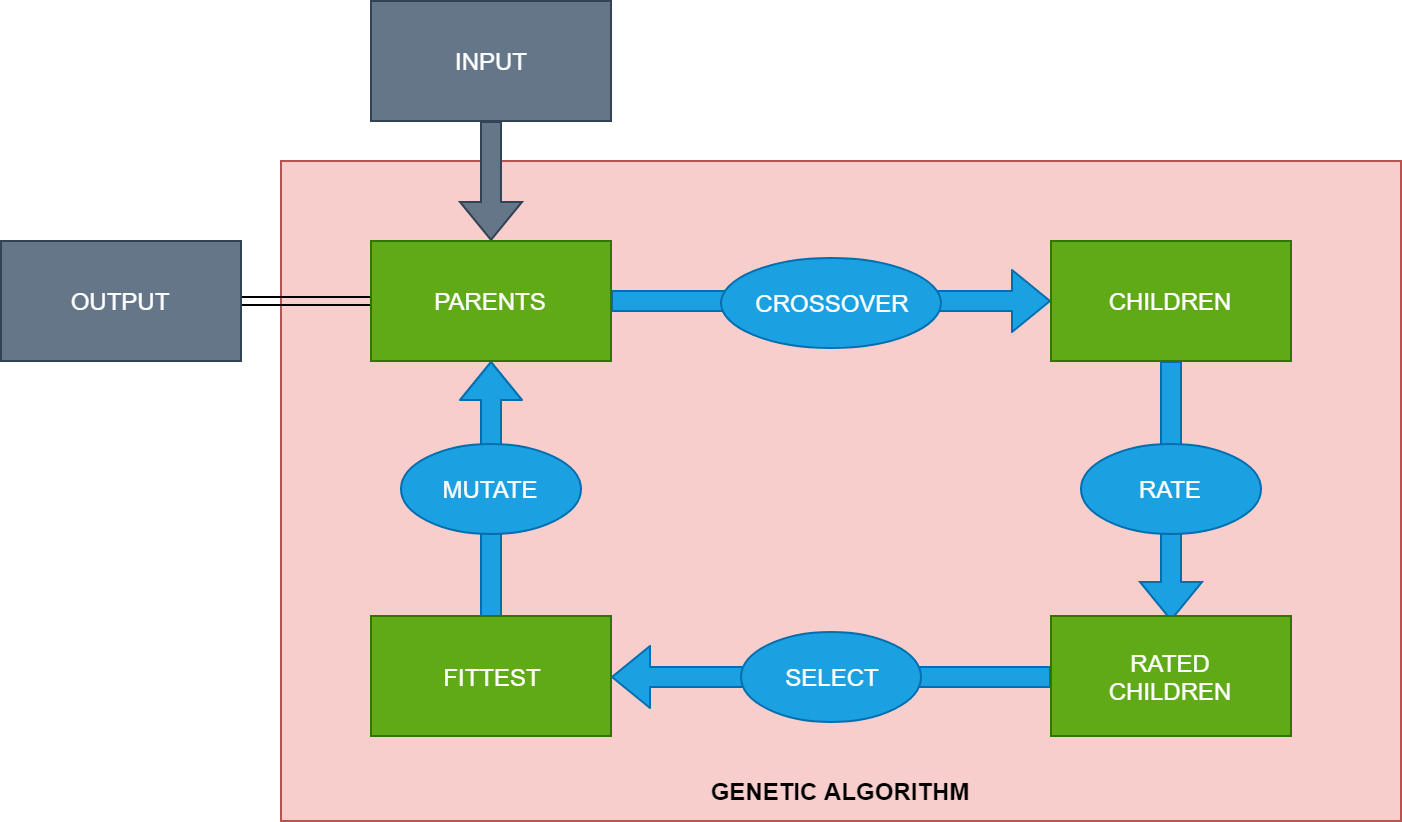
\includegraphics[width=\textwidth]{Fotos/App_structure.png}
	\caption{Global algorithm flow sketch.}
	\label{fig:App_structure}
\end{figure}


The program will end after a certain number of generation is reached. This amount is one of the elements from the input alongside the number of parents N.



\subsection{The crossover process} \label{sec:crossover}
It is important that the crossover of two songs happens in a consistent random way. The element (note, chord or rest) with the highest offset (time unit) of the resulting song cannot be higher than the maximum of the highest offset of the element of the pair. So we get the following equation that has to be correct every time we have paired song A with song B:
\[ Highest(AB) \leq Max(Highest(A),Highest(B))\]
With A and B the list of elements of song A and song B, respectively and AB the list of elements of the song AB that is a result of the crossing of song A and song B.
\\\\
This process is repeated multiple times during the execution, every song in a group must be paired with every other song. So we get for \(N\) parents \( \frac{N * (N-1)}{2} \) children.

\subsubsection{The crossover algorithm}
There are some assumptions we made that need to be discussed before moving on to the details of the algorithm. Both song A and song B have the same amount of measures and they are not empty. The reason for this is that all the elements in a song can be considered when crossing. For example, if song A has a length of 13 measures and song B a length of 17 measures. The elements of song B between measures 14 and 17 are left without a corresponding measure from measure A. To make it easier we cut every song in the beginning to an equal number of measures.  
\\\\
On listing \ref{code:crossover} a simple version of the crossover function's is visible in Python code.
\begin{lstlisting}[language=Python,caption={Simplified version of the crossover function},captionpos=b,label=code:crossover]
# INITIAL VALUES
cross_A = parentA.notes #Element list from parent song A
cross_B = parentB.notes #Element list from parent song B
list = [] #resulting list
indexA = 0 #index number in element list of song A
indexB = 0 #index number in element list of song B

For elements in A or B:

	choice = random.random()
	if choice > 0.5:
		# Swap lists 
		temp = cross_A
		cross_A = cross_B
		cross_B = temp
		temp = indexA
		indexA = indexB
		indexB = temp
	
	#Select the element from list A and copy to resulting list
	note = cross_A[indexA]
	new_note = copy.deepcopy(note)
	list.append(new_note)
	
	#Set list B's index to the next item at next offset
	currentoffsetB = cross_B[indexB].offset
	nextoffsetB = cross_B[indexB + 1].offset
	while nextoffsetB <= currentoffsetB:
		indexB += 1
		nextoffsetB = cross_B[indexB + 1].offset
	
	indexA+= 1 #next item index
	
	#adding elements from list A until list B's element is reached
	note = cross_A[indexA]
	next_note = cross_A[indexA+1]
	while next_note.offset < nextoffsetB :
		new_note = copy.deepcopy(note)
		list.append(new_note)
		indexA += 1
		note = cross_A[indexA]
		next_note = cross_A[indexA+1]
		
	if next_note.offset == nextoffsetB and 
			note.offset < next_note.offset:
		new_note = copy.deepcopy(note)
		list.append(new_note)
		indexA += 1
	
	
	#check if lists B's index is far enough
	currentoffset = cross_A[indexA].offset
	while cross_B[indexB].offset < currentoffset:
		indexB += 1

	
\end{lstlisting}
To fully explain the crossover algorithm, we will use an example. Say we have the parent songs A and B. Both A and B are filled with elements that are one of the following musical elements: note, chord or rest. These musical elements all start at some point in time, we call this unit the offset. Both of the lists have a maximum offset of 8. We copy elements to the resulting list based on these offsets of the elements. 
\\
To put it shortly: we iterate through the elements list, element by element and check with their offsets to decide if we copy the element or not. We make the assumption that these lists are sorted from the smallest to the largest offset. Figure \ref{fig:cross_init} illustrates the lists with elements on an offset scale. We temporarily leave out the exceptional cases where elements can have overlapping offsets.
\begin{figure}[H]
	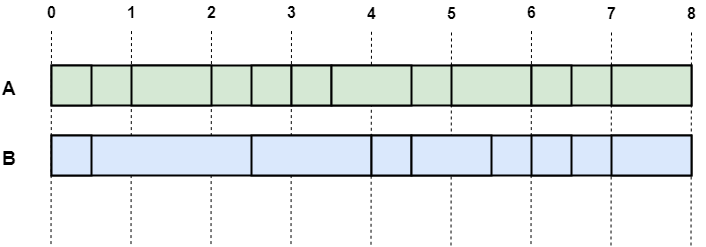
\includegraphics[width=\textwidth]{Fotos/crossover/init.png}
	\caption{Initial parent A and parent B.}
	\label{fig:cross_init}
\end{figure}

We initially have an empty list, AB, where we are going to add elements in from song A or song B. The first step is to randomly choose from which song's list we should pick the next element. Say we pick from song A and we add this element to AB. We get the following result shown on figure \ref{fig:cross_1}. 

\begin{figure}[H]
	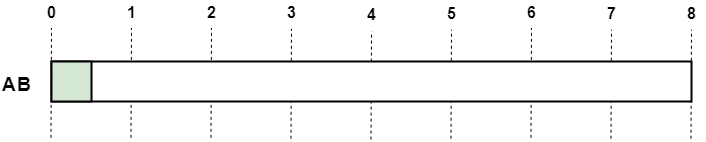
\includegraphics[width=\textwidth]{Fotos/crossover/first.png}
	\caption{List AB after 1 iteration, last choice = A.}
	\label{fig:cross_1}
\end{figure}

We then move to the next element of B and A where we have to make yet another choice. Now we are at the elements of A and B that are found on offset 0.5. Here we choose the element from list B and add it to AB. The chosen element starts at offset 0.5 and ends at offset 2.5, so we have to move our position to offset 2.5 and make a new choice. While moving our position, notice that we left out the elements in list A between 0.5 and 2.5. Briefly said, we choose song B during this interval.

\begin{figure}[H]
	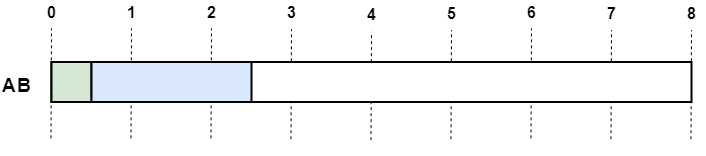
\includegraphics[width=\textwidth]{Fotos/crossover/2nd.png}
	\caption{List AB after two iterations, last choice = B.}
	\label{fig:cross_2}
\end{figure}

Let us choose the next element from song A. We can clearly see that song B's next element is at offset 4.0. This means that all the elements from song A until offset 4.0 can be copied to list AB. The elements of A at offset 2.0, 2.5 and 3.0 can be copied. The element starting on offset 3.5, however, will not be added because it ends on offset 4.5. This element will be considered in the next choice. Figure \ref{fig:cross_3} illustrates our current situation of song AB.

\begin{figure}[H]
	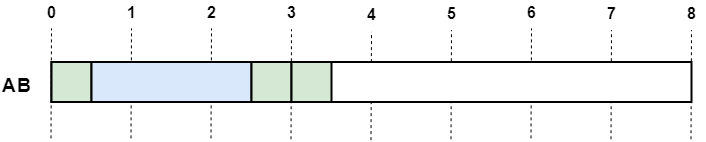
\includegraphics[width=\textwidth]{Fotos/crossover/3th.png}
	\caption{List AB after three iterations, last choice = A.}
	\label{fig:cross_3}
\end{figure}
Next up we select the element from B at offset 4.0 instead of the element from A at offset 3.5. We end up getting a gap between 3.5 and 4.0 just like shown on figure \ref{fig:cross_4}. This gap will be filled later with a rest.

\begin{figure}[H]
	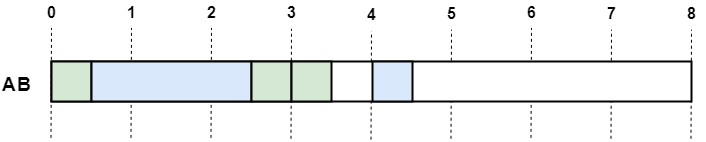
\includegraphics[width=\textwidth]{Fotos/crossover/4th.png}
	\caption{List AB after four iterations, last choice = B.}
	\label{fig:cross_4}
	
\end{figure}
For the remaining part, we follow the same process over and over again. Say we make the following choices: at offset 4.5 elements from B until 6.0, at offset 6.0 elements from A until 7.0 and at last at offset 7.0 elements from B until 8.0 the end. These past choices are illustrated at figure \ref{fig:cross_5}, \ref{fig:cross_6} and \ref{fig:cross_7} in that order.

\begin{figure}[H]
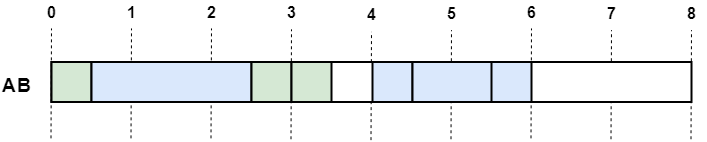
\includegraphics[width=\textwidth]{Fotos/crossover/5th.png}
\caption{List AB after five iterations, last choice = B.}
\label{fig:cross_5}
\end{figure}

\begin{figure}[H]
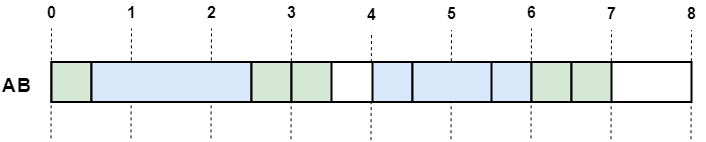
\includegraphics[width=\textwidth]{Fotos/crossover/6th.png}
\caption{List AB after six iterations, last choice = A.}
\label{fig:cross_6}
\end{figure}

\begin{figure}[H]
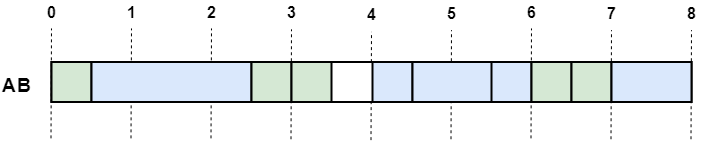
\includegraphics[width=\textwidth]{Fotos/crossover/last.png}
\caption{List AB after seven iterations, last choice = B.}
\label{fig:cross_7}
\end{figure}

Now that we have demonstrated the algorithm with an example, there is still one thing remaining to discuss. What do we do with elements that have the same offset? We simply copy them alongside each other. So let us say there are two elements at offset 0.0, we copy them both. They are both considered to be part of a group that shares the same offset. Instead of copying individual elements, we copy groups of elements that share the same offset. 

\subsection{Rating strategies \& functions} \label{sec:rating}

In this part of the application, the songs are getting rated one by one. The rating consists of a certain amount of sub-ratings that add up to a total rating. The lower the number of this total score, the better a song is considered and the more likely it will be chosen for repopulation. Every sub-rating consists of a score and a weight. The score is the result of a comparison between the to be rated song's score and an optimal score. This optimal score can be predefined by music theory, for example, but does not have to be. More about this will follow later. The weight represents the amount of impact the score will have on the final result of the sub-rating. 
\\
Let us demonstrate this as follows: suppose there are only three sub-raters that have the following functions as their score calculators that calculate a score and compare them to the optimal: f(x), g(x) and h(x). We already explained that every sub-rater has some sort of a multiplier: its weight. Let A, B and C be the weights related to f(x), g(x) and h(x) in that order. The total rating R(x) for a song x would be defined by the following equation:  \[ R(x) =  A * f(x) + B * g(x)  +  C * h(x)  \]
There are without a doubt more than only three sub-raters, we can now define a new equation that takes all the existing sub-raters into account: 
\[ R(x) = \sum_{S=1}^{n} S_{score} * S_{weight} \   \text{  (with S as sub-rater)}\] 
\\
In words: a song's total rating is equal to the sum of every sub-rater's score for that song, multiplied by that sub-rater's weight.
\\\\
This is very similar to the approach used in "Generation of music through genetic algorithms" \cite{genmusicbach}. The variation we add on top is the sub-rater's weights. Because of these weights, we are able to adjust the impact of every sub-rater towards our wishes which results in customized experience. They also use fixed optimal scores but we do not as we will explain later. In "A Genetic Algorithm for composing music" \cite{genetic} they use similar concepts as we do with weights. They use it as some sort of influence. They change these weights during the execution of the program.


\subsubsection{Scores \& different strategies}
Because musical preference is considered to be subjective, we can not simply define elements that make music sound good in a way that works for every instance. It is and will be a personal choice. We can, however, use user preferences as an input. We defined a way to profile these preferences. We made it able to define different rating strategies in order to represent these diverse profiles. There are two core profiles: one that is based on music theory: TheoryBasedRatingStrategy and one that is based on user input: SampleBasedRatingStrategy. \\
\newline
Every sub-rating function compares the song's score of the particular subject the sub-rater is supposed to give a score, to that sub-rating's optimal score. For example: consider a sub-rater that gives a score to a song on the amount of uniqueness of the notes. Suppose the optimal score is that 30\% of the notes are unique. Now the sub-rater function calculates the score for the to be rated song and finds that 35\% of his notes are unique. At last, we compare these two value's and return a rating of 5\% which translates to 0.05. Now, the resulting rating of the sub-rater's is 0.05 multiplied by the sub-rater's weight. We can generalize this as follows:

\[ S(x) =  difference( f(x) ,optimalscore) * S_{weight} \]
with $ f(x)$ the sub-rater's score calculator, the optimal-score as a calculated or predefined value and $  S_{weight} $ the sub-rater's attached weight.
\newline
We can fill in the weights and the optimal scores based on different genres and styles of music into different strategies and use these objects as genre/style definitions. Strategies that are based on jazz music will have different weights and optimal scores as strategies that are based on classical music. The TheoryBasedRatingStrategy, for example, gives a song a rating based on predefined musical rules that are well-known to make music sound good.\\
A second and rather more interesting approach is to calculate these optimal scores based on a song. SampleBasedRatingStrategy takes a song as input, we define it as the "master song", and extracts as much possible musical data from a song to define every optimal score of every sub-rater. SampleBasedRatingStrategy will now rate songs better that have a similar structure as the master song. Now we give the possibilities to define specific song theory and use it as the perfect solution. These optimal scores based on the master are just scores that have been calculated by running the sub-rater functions on the master.

 
\subsection{General purpose sub-raters}
In this section, we will break down all of the sub-raters that are implemented as rating strategies. Every sub-rater will, of course, have his own weight and optimal score where it will be compared to (as mentioned before). We will consider the impact of those variables in another section. In this section, however, we explain the sub-raters functions and algorithms that calculate the song's score. 
\\\\
The general purpose sub-raters are sub-raters that do not necessarily need a master song. They can be used in a general way without a master song, the optimal scores are predefined.


\subsubsection{Scale correctness score} \label{subrater:scale_corr}
With the help of the music21 library, we are able to analyze a song's match rate with the closest scale it follows. So what this means is that we can analyze which scale a song's notes differ the least from and create a rating based on that particular scale. This rating is a relative ratio between 0 and 1. The Scale Correctness score for a song x is calculated by the following equation:

\[ ScaleCorrectness(x) = 1 -  \frac{\textit{Number of matching unique notes}}{\textit{Total amount of unique notes}}  \]
or:

\[ ScaleCorrectness(x) =  \frac{\textit{Number of not-matching unique notes}}{\textit{Total amount of unique notes}}  \]


\subsubsection{Zipf's law distance scores}
Zipf's law definition: 
\begin{quotation}
	"Zipf's law is an empirical law formulated using mathematical statistics that refers to the fact that many types of data studied in the physical and social sciences can be approximated with a Zipfian distribution, one of a family of related discrete power law probability distributions" \cite{Zipfslaw}.
\end{quotation}

In "Zipf's Law, Music Classification, and Aesthetics" \cite{Zipfslaw_paper} was explained that music that followed Zipf's law, or were closer to it than other songs, were more likely to be preferred by the majority of an audience. This means that Zipf's law can be a useful metric to rate a song's quality. Applying Zipf's law on a distribution will result in a Zipfian distribution.
\\\\
A Zipfian distribution is a distribution where the 2nd highest occurring element, occurs 1/2 times the number of occurrences of the highest occurring element, the 3rd highest occurring element, occurs 1/3 times the number of occurrences of the highest occurring element and so on. Suppose L is the number of occurrences of the most popular element. For every element E, with rank R (position of the element on the list of unique elements ordered by its frequency of appearance), the amount of occurrences is defined by the following function:

\[ Occurences(E) =  \frac{1}{R} * L  \]

For every unique element the previous function is used to create a perfect Zipfian distribution.

\paragraph{Wasserstein distance}\mbox{}\\
Before moving on we need to handle an important concept that we use to calculate the distance between distributions. The Wasserstein distance, $Wd(u,v)$, between the distributions $ u $ and $ v $ is \cite{wasserstein_python}:


\[ Wd(u,v) =  inf_{\pi \in \Gamma (u,v)} \int_{\mathbb{R} X \mathbb{R} } ||x-y|| d\pi(x,y) \] 
The "inf" in the formula stands for infimum, which indicates that we only consider the minimal cost.
We can clarify this equation with an existing example from "Towards Polygonal Mesh Generation With
Generative Adversarial Networks" \cite{wasserstein_paper}, say we have two distributions P and Q: 

\[ P =  {3,2,1,4}  \]
\[ Q =  {1,2,4,3}  \]

The distance of these distributions would be $||3-1|| + ||2-2|| + ||1-4|| + ||3-4|| = 5$. But we only pair the corresponding elements based on their index in the distribution. The Wasserstein distribution pairs element on each possible way ($\mathbb{R} X \mathbb{R}$) and calculates their distance and gives as result only the lowest value. The combination that has the lowest value will be $||1-1|| + ||2-2|| + ||4-4|| + ||3-3|| = 0$. We can clearly see that there is a major difference between the combinations of the elements both formulas consider. We use the Wasserstein distance in our case because we are not interested in the order of the elements. We are interested in how little effort is needed to transform one distribution into one other, which is exactly what the Wasserstein distance stands for.


\paragraph{Pitches}\mbox{}\\
We create a list of all pitches that occur in a song and consider it as a distribution. We create another list that has a Zipfian distribution with the exact same given pitches. Now we have the song's pitch distribution and its perfect Zipfian distribution. 
\\\\
To compare both distributions we calculate the Wasserstein distance between them which results in an absolute metric. In order to transform the absolute to the relative, we generate the worst-case scenario where the distance would be equal to the maximum possible distance. This is achieved by the comparison with a uniform distribution. By calculating the Wasserstein distance between the Zipf's and this new uniform distribution, we create an absolute number that represents the maximum distance. This absolute limit allows us to get a relative rating, Zipf's law distance rating for pitches Zp, out of the absolute distance. 
We get the following equation:

\[ ZipfPitch(x) =  \frac{WD(\textit{Distribution of song's pitches},\textit{Ziphian Distribution of song's pitches})}{WD(\textit{Uniform Distribution of song's pitches},\textit{Ziphian Distribution of song's pitches})} \]


\paragraph{Intervals}\mbox{}\\
We can do the same for the intervals between notes of the song as we did with the pitches which results as the following equation:

\[ ZipfInterval(x) =  \frac{WD(\textit{Distribution of song's intervals},\textit{Ziphian Distribution of song's intervals})}{WD(\textit{Uniform Distribution of song's intervals},\textit{Ziphian Distribution of song's intervals})} \]

Zipf's law can also be considered with intervals as it did with pitches.


\subsubsection{Neighbour pitch score}\label{sec:rater:neighbourpitch}
This rating represents the amount of wrong or unpleasant intervals. Unpleasant intervals are defined by genre or by the master song. We measure the number of steps needed to raise or lower a previous note to get the current note. For example, to reach the note C6 from G5, you need to lower the song by 5 semitones which is interpreted as -5 in our system. We have defined a minimum and a maximum limit (by genre or by a master) thus we can recognize unpleasant intervals that are outside of this domain. The neighbour pitch rating actually rates the amount of the occurrences of these unpleasant intervals. The following equation emerges for the neighbour pitch rating $ NeighbourPitch(x) $ of a song x:

\[ NeighbourPitch(x) = \frac{\textit{Number of unpleasant intervals}}{\textit{Total number of intervals} } \]


\subsubsection{Melody based scores}
\paragraph{Melody direction score}\mbox{}\\
This score is a number between 0 and 1 that represents the direction of the melody. If the number is higher than 0.5, the direction is of the melody is going upwards, else it is going downwards. We can calculate this score by comparing the amount of upwards intervals (positive semitones) to all the intervals. The melody direction score of a song x is defined as:

\[ MelodyDirection(x) = \frac{\textit{Number of upwards intervals}}{\textit{Total number of intervals} } \]


\paragraph{Direction stability score}\mbox{}\\
This score gives a score of the amount of the times the direction of the melody changes. By testing if the direction of the current interval is the same as the previous we determine these changes. The direction stability score of a song x is defined as:

\[ DirectionStability(x) = \frac{\textit{Number of direction changes intervals}}{\textit{Total number of intervals} } \]


\paragraph{Unique pitches score}\mbox{}\\
This score represents the rate of uniqueness of the pitches of the song. The Unique pitches score of a song x is defined as:

\[ UniquePitches(x) = \frac{\textit{Number of uniques pitches}}{\textit{Total number of pitches} } \]


\subsubsection{Measure relations \& repetition scores} \label{sec:measure_rel}
This is an advanced sub-rater that builds up the basis for other upcoming sub-raters from the master based sub-raters in section \ref{sec:master_based_subrater}. In order to define repetition, we need to compare certain parts to each other. These parts can have relations towards others for example, two not overlapping parts A and B scattered over the song that are 90\% similar to each other. The size of these parts are important and can vary among different parts that have different relations with each other and so on. To keep this simple and manageable, we defined the parts to have equal lengths: 1 measure lengths. Instead of random parts in a song, we combine measures to each other. We eliminate the possibility of having repetitive parts or patterns over sizes that differ from the measure length.
\\\\
In this sub-rater, we first create a way to calculate a match rate between measures. We represent a measure as a list of strings in multiple dimensions. These dimensions are the following:
\begin{itemize}
	\item pitch,
	\item type,
	\item duration,
	\item offset,
	\item combined (combines pitch, type, duration and offset with each other),
	\item semitones.
\end{itemize}
Here is a full example of a measure represented in the just discussed way:

\[ types: [X, X, N, X, X, N] \]
The types list represents the types of the music elements (note as N, chord as X and rest as R) in the chronology they occur in the measure itself.

\[pitches: [G\sharp3G\sharp4, D3B2, C3, C5G4E\flat4, E\flat4G4C5, B4]\]
The pitches list represents the corresponding pitch(es) the musical elements have in the chronology they occur in the measure itself.

\[durations: [half, quarter, eighth, eighth, eighth, eighth] \]
The durations list represents the duration of the musical elements also in the chronology they occur in the measure.

\[offsets: [0.0, 1.0, 2.0, 2.5, 3.0, 3.5] \]
The offsets list represents the start time of every element that occurs in the measure. This list is also chronologically ordered.

\[ combined: [XG\sharp3G\sharp4h0.0, XD3B2q1.0, NC3e2.0, XC5G4E\flat4e2.5, XE\flat4G4C5e3.0, NB4e3.5] \]
The list combined is a combination of the types, pitches, durations and offsets.

\[semitones: [-6, -2, 24, -9, 8] \]
This list represents the semitones values of the intervals between the notes and chords. Rests are skipped.
\\\\
All these lists give the possibility to match measures in a song with others based on a specific dimension or the complete packet. This allows us to recognize patterns in a song and give a kind of pattern rating. The higher the match rate of a measure with others, the more likely it is that there is a pattern in the song that repeats itself somewhere. We used the fuzzy-wuzzy library \cite{FuzzyWuzzy} matching in order to obtain a score we can use for our rating purpose. The library uses the Levenshtein distance \cite{Levenshtein_distance} to get a ratio between 0 and 1 that represents the similarity between the two lists of the measures. As the definition goes: 
\begin{quotation}
	"The Levenshtein distance between two words is the minimum number of single-character edits (insertions, deletions or substitutions) required to change one word into the other."
\end{quotation}

Let us demonstrate this process with an example. Say we have the following types list of two measures:
\[ types1: [X, X, N, X, R, N] \]
\[ types2: [X, N, N, X, R, N] \]
We will get a 97\% of a match rate between $types1$ and $types2$. However, there are more dimensions in a measure than only the types, that is why we introduced a way to compare the big picture with the combined list. We will use an example of two measures, A and B, that are very similar. These measures are taken from the Godfather theme song. Measure A is the 9th, measure B the 10th. We illustrated these measures on figure \ref{fig:GF_measures}.

\begin{figure}[H]
	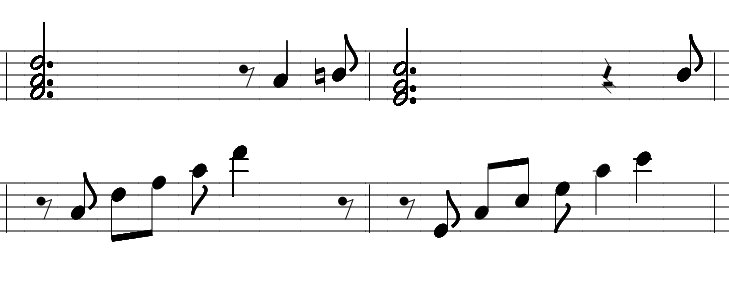
\includegraphics[width=\textwidth]{Fotos/measures/GF_9-10.png}
	\caption{The 9th and 10th measure of the Godfather theme song.}
	\label{fig:GF_measures}
\end{figure}

We examine and compare them to each on all the dimensions by creating the according to lists and matching them.

\[\textit{TYPES}\]
\[A: [X, N, N, N, N, N, N, N] \]
\[B: [X, N, N, N, N, N, N, N] \]
\[\textit{types match rate}: 100\% \]


\[\textit{PITCHES}\]
\[A: [E\flat4C5G4, G2, C3, E\flat3, G3, C4, E\flat4, B\flat4] \]
\[B: [D5G\sharp4F4, C3, F3, G\sharp3, C4, F4, G\sharp4, B4] \]
\[\textit{pitches match rate}: 74\% \]


\[\textit{DURATIONS}\]
\[A: [complex, eighth, eighth, eighth, eighth, quarter, quarter, eighth] \]
\[B: [complex, eighth, eighth, eighth, eighth, quarter, quarter, eighth] \]
\[\textit{durations match rate}: 100\% \]


\[\textit{OFFSETS}\]
\[A: [0.0, 0.5, 1.0, 1.5, 2.0, 2.5, 3.0, 3.5]\]
\[ B: [0.0, 0.5, 1.0, 1.5, 2.0, 2.5, 3.0, 3.5] \]
\[\textit{offsets match rate}: 100\% \]


\[\textit{SEMITONES}\]
\[ A: [-20, 5, 3, 4, 5, 3, 7] \]
\[ B: [-26, 5, 3, 4, 5, 3, 3]\]
\[\textit{semitones match rate}: 91\% \]


\[\textit{COMBINED}\]
\[ A: [XE\flat4C5G4c0.0, NG2e0.5, NC3e1.0, NE\flat3e1.5, NG3e2.0, NC4q2.5, NE\flat4q3.0, NB\flat4e3.5]\]
\[ B: [XD5G\sharp4F4c0.0, NC3e0.5, NF3e1.0, NG\sharp3e1.5, NC4e2.0, NF4q2.5, NG\sharp4q3.0, NB4e3.5]\]
\[\textit{combined match rate}: 85\% \]





As you can see, these measures have a very high match rate. But it is important to notice the following: if we combine the first four lists (types, pitches, durations, offsets) of each song we get the combined list. Matching these combined lists with each other results in a rate of 85\%. On the other hand, if we calculate the mean of the four lists rating we get a different result: $(100 +75+100+100) /4 = 93.75 $. 93.75\% Is much higher than 85\%. This is exactly the reason why we cared about a combined match rate. After analyzing the values of these lists, we came to the conclusion that even if some lists have a very high rate, this does not mean the measures match well with each other. We are forced to look at the complete picture in order to decide the rate of resemblance between measures.
\\\\
After analyzing the comparison of each measure with others by listening to them and comparing the repetition to the scores, we defined some measure types. These types were completely defined by ear and do not have a theoretical background to support them. We made a distinction between the following relation types between two measures: strong bindings, normal bindings, weak bindings, garbage bindings. We use the term binding because we consider that two measures have been bonded together by a rate. A strong binding is of a stronger type than the normal binding, a normal binding is of a stronger type than the weak binding and a weak binding is of a stronger type than the garbage binding.
\\\\
Strong bindings are bindings where repetition is very likely to be noticeable between both measures. For two measures to be strongly bonded we noticed that the following rules with threshold 80\% need to be true:
\begin{enumerate}
	\item At least three of the following ratios have to be over the threshold: 80\%: 
			\begin{enumerate}
				\item types match rate
				\item pitches match rate 
				\item offsets match rate - 5
				\item durations match rate - 5
				\item semitones match rate 
			\end{enumerate}
	
	\item $(semitones match rate + combine match rate) / 2 \geq 80 (= threshold)$
\end{enumerate}
In the Godfather theme song, we discovered some measures that were strongly bonded to each other. We only consider the first 16 measures. We represented these bindings on the graph shown on figure \ref{fig:GF_strong_graph}.


\begin{figure}[H]
	\includegraphics[width=\textwidth]{Fotos/bindings_graph/Godfather_16_strong.png}
	\caption{Graph representing strong bindings between measures: each node is a measure with its number inside, each edge represents the strength of matching rate between them.}
	\label{fig:GF_strong_graph}
\end{figure}

We can clearly see that there are groups of strong bindings. The measures that are not strongly bonded have no connection with each other, we just want to illustrate the level of repetition of in groups. The graph representation has been very useful to determine the rules that type a binding to be strong, normal, weak or garbage.
\\\\
Normal bindings are bindings where repetition is less likely to be noticeable compared to strong between both measures. For two measures to be normally bonded they would have the same rules with a different threshold: 70\%. Also, a normal binding must not be a strong binding, so the values compared to the threshold are less than 80\%. When we analyzed the Godfather theme song for normal measures, we were able to construct the graph on figure \ref{fig:GF_normal_graph}.

\begin{figure}[H]
	\includegraphics[width=\textwidth]{Fotos/bindings_graph/Godfather_16_normal.png}
	\caption{Graph representing normal bindings between measures: each node is a measure with its number inside, each edge represents the strength of matching rate between them.}
	\label{fig:GF_normal_graph}
\end{figure}
These normal bonded measures had some sort of coherence with each other. They tend to be like each other but do most likely not give a feeling of repetition. As you can see the graph has more nodes and has more edges relative to the strong bindings graph on figure \ref{fig:GF_strong_graph}.
\\\\
Last but not least, we have two bindings to discuss: weak bindings and garbage bindings. The weak bindings have as threshold 55\% and the garbage threshold has no threshold. They represent everything that is left over, in other words, everything below 55\%.

\begin{figure}[H]
	\includegraphics[width=\textwidth]{Fotos/bindings_graph/Godfather_16_weak.png}
	\caption{Graph representing weak bindings between measures: each node is a measure with its number inside, each edge represents the strength of matching rate between them.}
	\label{fig:GF_weak_graph}
\end{figure}

On figure \ref{fig:GF_weak_graph} we can see that a lot of measures are weakly bonded with each other. These bindings have little resemblance with each other. On this graph, we see that all the measures have weak bindings with each other. This gives us a good indication of how likely it is that the measures of a song can have big differences.

\begin{figure}[H]
	\includegraphics[width=\textwidth]{Fotos/bindings_graph/Godfather_16_garbage.png}
	\caption{Graph representing garbage bindings between measures: each node is a measure with its number inside, each edge represents the strength of matching rate between them.}
	\label{fig:GF_garbage_graph}
\end{figure}

On figure \ref{fig:GF_garbage_graph} we can see that 11 out of 16 measures have garbage bindings with other measures. This means that 5 measures have no garbage bindings. This is a useful way to analyse at a song to compare it with other songs. This allows us to look how the measures are bonded to each other and if it is possible to have measures that have some no garbage bindings. This means we can rate if a song has measure with only high bondings (weak, normal, strong).

\paragraph{Measure bindings rate}\mbox{}\\
This measure bindings rate is calculated based on the amount of strong, normal, weak and garbage bindings between measures. So we calculate each type occurrence rate in the song and compare it to the optimal rates. Let us make that last clear. For $M$ measures there are \( \frac{M  (M-1)}{2} \) bindings, if from these $M!$ bindings $s$ number of them are strong, the strong bindings rate would be $\frac{2s}{ M  (M-1)  }$. For each type, we calculate the rates that represent their share for all of the bindings \( \frac{M  (M-1)}{2} \). For each song $x$ with $M$ measures, the measure bindings rate is illustrated as follows:
First, we calculate the bindings rate of each type:


\[ StrongBindingsRate(x) = \frac{\textit{2s}}{M  (M-1)} \]
with s the number of strong bindings,

\[ NormalBindingsRate(x) = \frac{\textit{2n}}{M  (M-1)} \]
with n the number of normal bindings,

\[ WeakBindingsRate(x) = \frac{\textit{2w}}{M (M-1)}   \]
with w the number of weak bindings,

\[ GarbageBindingsRate(x) = \frac{\textit{2g}}{M (M-1)} \]
with g the number of garbage bindings.
\\\\
Next, we compare each of the rates to the optimal score by calculating the difference between the optimal rates. We eventually get the following:

\[MeasureBindingsRating(x) = Difference( StrongBindingsRate(x) , OptimalStrongBindingsRate) \]
\[+ Difference( NormalBindingsRate(x) , OptimalNormalBindingsRate) \]
\[+ Difference( WeakBindingsRate(x) , OptimalWeakBindingsRate) \]
\[+ Difference( GarbageBindingsRate(x) , OptimalGarbageBindingsRate) \]
 

Notice that this sub-rater is different than others, we calculate the difference earlier on with the optimal scores instead of leaving as the final step. The reason for this is that all of the types rates have an optimal rate that we need to compare to. Afterward, we can add up the difference between them to get a whole correctness ratio per type. Adding up those differences will result in the measure bindings rating.

\paragraph{Measures types rate}\mbox{}\\ \label{sec:measure_type}
This rating is based on the measure itself instead of the bindings. Every measure can be categorized by its best possible measure bonding. Let us demonstrate this last with the Godfather theme song hence we already analyzed the bindings in it. On figure \ref{fig:GF_strong_graph} we can clearly see that the measures 1,2,3,5,7,6,9,10 and 14 have at least one strong binding. This means their strongest binding with another measure is of the type strong. 
The strong measure rate is hereby equal to the number of measures with its strongest binding type strong $s$ divided by the number of measures M:

\[ StrongMeasureRate(x) = \frac{\textit{s}}{\textit{M} } \]
In our example, there are 9 measures that have as their strongest binding a strong binding out of 16 measures thus $StrongMeasureRate$ of the Godfather song is $\frac{9}{16} =  0.5625$.
\\\\
If we look at the normal bindings on figure \ref{fig:GF_normal_graph} we see that all the measures have a normal binding with at least one measure. This means that all measures have at least normal strength bindings. But this does not mean that the strongest binding of these measures is of the normal strength type. Only the measure with their strongest measure binding being normal must be considered, all the measures that have a strong binding must be eliminated from the count. The normal measure rate is hereby equal to the number of measures with as strongest bindings type normal $n$ divided by the number of measures M:

\[ NormalMeasureRate(x) = \frac{\textit{n}}{\textit{M} } \]
In the Godfather theme song, there are 7 measures out of 16 measures that have as their strongest binding a normal binding, thus $NormalMeasureRate$ of the Godfather song is $\frac{7}{16} =  0.4375$.
\\\\
The weak measure rate is hereby equal to the number of measures with as strongest bindings type weak $w$ divided by the number of measures M:
\[ WeakMeasureRate(x) = \frac{\textit{w}}{\textit{M} } \]
In the Godfather theme song, there are 0 measures that have as their strongest binding a weak binding thus $WeakMeasureRate =  0.0$.
\\\\
The garbage measure rate is equal to the number of measures with as strongest bindings type garbage $g$ divided by the number of measures M:
\[ GarbageMeasureRate(x) = \frac{\textit{g}}{\textit{M} } \]
In the Godfather theme song, there are 0 measures that have as their strongest binding a garbage binding thus $GarbageMeasureRate =  0.0$.
\\\\
What do these results say about the Godfather theme song? Having a $WeakMeasureRate =  0.0$ and a $GarbageMeasureRate =  0.0$ means that all of the measures  have some sort of bond with each other. There cannot be an outcast of a measure that has nothing in common with any of the measures, not according to the Godfather theme song. 
\\\\
Finally, we have to compare these rates to an optimal score rate just like we did to calculate the $MeasureBindingsRating$ in the previous section. We compare each of the rates to the optimal score by calculating the difference between the optimal rates. We eventually get the following:

\[MeasureTypesRating(x) = Difference( StrongTypeRate(x) , OptimalStrongTypeRate) \]
\[+ Difference( NormalTypeRate(x) , OptimalNormalTypeRate) \]
\[+ Difference( WeakTypeRate(x) , OptimalWeakTypeRate) \]
\[+ Difference( GarbageTypeRate(x) , OptimalGarbageTypeRate) \]



\subsection{Master based sub-raters} \label{sec:master_based_subrater}
These sub-raters are special purpose raters. These sub-raters can only be used if the music theory is determined by a sample song called the master. We only can calculate the rating in this section by comparing the songs from the population with the master. That is why these sub-raters are considered to be special purpose. We need optimal scores to rate a song. These optimal scores can only be extracted by a master song.
\subsubsection{Relative ratings}\label{sec:relratings}
\paragraph{Measure based sub-rating}\mbox{}\\ \label{sec:relmeasurebasedratings}
These sub-ratings are based relative to the master song. These relative ratings are calculated on a measure size and summed up afterwards to represent the whole song. What we actually calculate is how the measures relate to one and another in the song. 
\\\\
Let us demonstrate this with an example: say we want to look at the behavior relation of the types of measures in the song on a measure size bases. So for the first measure, we collect their resemblance with the others. We calculated this ratio previously and stored them per measure. The list we get for the first measure $m_1$ looks like the following:

\[\textit { first measure types relation list of our to be rated song, TypeRelations $m_1$}:\]
 \[[77, 85, 89, 85, 85, 77, 83, 88, 77, 82, 83, 92, 86, 85, 86]\]
Notice that the size of the list is 15 hence there are 16 measures. Obviously, we are not interested in the comparison of the measure with itself. The lists have the following meaning: The first element in the list $77$ is a rate that represents the resemblance between our first measure with the second, the second element in the list $85$ is a rate that represents the resemblance between our first measure with the third and so on. Notice that this list only represents the relations of measure one with the others and not all measures with each other.
\\\\
The following action is to compare this list with its optimal. The optimal is the same list calculated for the master song. Say we have as the master song the Godfather theme, its Types Relations list of measure 1,  $g_1$ , looks like this:
\[ \textit {first measure TypeRelations of Godfather theme song, TypeRelations $g_1$} \]
\[[100, 100, 77, 68, 73, 68, 80, 68, 68, 71, 80, 66, 73, 63, 68]\]
Now we compare them to each other by using the Wasserstein distance, this means the order of occurrence is not taken into account because the Wasserstein distance ignores it. We are only interested in the quality of the relations. Remember that the Wasserstein distance gives an absolute value that we need to make relative. We calculate some maximum possible distance to use as a limit as follows: notice that the values in the list are values between 0 and 100. If we take TypeRelations list of the Godfather theme song and for every element, we replace it with the maximal distance possible we will get the following list:
\[ \textit {complement values of the first measure TypeRelations of Godfather theme song, ComplementTypeRelations $g_1$} \]
\[[0, 0, 0, 0, 0, 0, 0, 0, 0, 0, 0, 0, 0, 0, 0]\]
The maximum distance of the first element $100$ is $0$, the maximum distance of the second element $100$ is $0$, the maximum distance of the third element $77$ is $0$ and so on. We also calculate the Wasserstein distance of the first measure TypeRelations of Godfather theme song with the limit distance of the first measure TypeRelations of Godfather theme song.
\\\\
The rating of the first measure $m_1$ will be calculated with the following equation:

\[ \textit{TypeRelationsRating($m_1$) } = 
\frac{WD(\textit{TypeRelations $m_1$},\textit{TypeRelations $g_1$})} {WD(\textit{ComplementTypeRelations $g_1$},\textit{TypeRelations $g_1$})} \]
We calculate this value for each measure $m_n$ in the song $x$ and the divide it by the number of measure $M$ in the song, we will get the types distance sub-rater's equation:


\[ \textit{TypeDistanceRating($x$) } =  \frac{1}{M}\sum_{n=1}^{M}
\frac{WD(\textit{TypeRelations $m_n$},\textit{TypeRelations $g_n$})} {WD(\textit{ComplementTypeRelations $g_1$},\textit{TypeRelations $g_n$})} \]

Now we have calculated the relative type distance rating of the song $x$. We can do the same for the other dimensions.\\\\
Offsets distance sub-rater's equation:
\[ \textit{OffsetDistanceRating($x$) } =  \frac{1}{M}\sum_{n=1}^{M}
\frac{WD(\textit{OffsetRelations $m_n$},\textit{OffsetRelations $g_n$})} {WD(\textit{ComplementOffsetRelations $g_1$},\textit{OffsetRelations $g_n$})} \]
\\\\
Pitches distance sub-rater's equation:
\[ \textit{PitchDistanceRating($x$) } =  \frac{1}{M}\sum_{n=1}^{M}
\frac{WD(\textit{PitchRelations $m_n$},\textit{PitchRelations $g_n$})} {WD(\textit{ComplementPitchRelations $g_1$},\textit{PitchRelations $g_n$})} \]
\\\\
Durations distance sub-rater's equation:
\[ \textit{DurationDistanceRating($x$) } =  \frac{1}{M}\sum_{n=1}^{M}
\frac{WD(\textit{DurationRelations $m_n$},\textit{DurationRelations $g_n$})} {WD(\textit{ComplementDurationRelations $g_1$},\textit{DurationRelations $g_n$})} \]
\\\\
Semitones distance sub-rater's equation:
\[ \textit{SemitoneDistanceRating($x$) } =  \frac{1}{M}\sum_{n=1}^{M}
\frac{WD(\textit{SemitoneRelations $m_n$},\textit{SemitoneRelations $g_n$})} {WD(\textit{ComplementSemitoneRelations $g_1$},\textit{SemitoneRelations $g_n$})} \]

All of the sub-rater's equations above will be multiplied with its own corresponding weight to get their final impact rating.

\paragraph{Types distribution rating}\mbox{}\\
There is still one rating left: Types distribution rating. This rating compares the occurrences rates of the different types and compares them with the occurrence rate of the master. Say the we have the following occurrence rate for the types of son $x$: $notes$ = $0.5$, $chords$ = $0.4$ and $rests$ = $0.1$. We get the following equations: 
\[ NotesOccurenceRate(x) = \frac{\textit{Number of notes of x}}{\textit{Total number of elements of x} } \]
\[ ChordsOccurenceRate(x) = \frac{\textit{Number of chords of x}}{\textit{Total number of elements of x} } \]
\[ RestsOccurenceRate(x) = \frac{\textit{Number of rests of x}}{\textit{Total number of elements of x} } \]
We compare these rates to the corresponding occurrence rates of the master by taking the positive difference between them. The sum of these differences will be the types distribution rating. The types distribution rating of a son $x$ with master $g$ is calculated by the following formula:

\[ TypesDistributionRate(x) = Difference( NotesOccurenceRate(x) , NotesOccurenceRate(g) \]
\[+ Difference( ChordsOccurenceRate(x) , ChordsOccurenceRate(g)) \]
\[+ Difference( RestsOccurenceRate(x) , RestsOccurenceRate(g)) \]


\subsubsection{Absolute Ratings}
In this section, we discuss sub raters that have a direct connection to the master song. We do not compare value calculated within the songs, we calculate this value by directly comparing the songs with each other. For example, instead of comparing the values received from comparing elements from the same song with the master, we directly compare elements from the song to the master. 


\paragraph{Element count rating}\mbox{}\\
This rater is based on the amount of elements in a song compared to the master song. This sub-rating is calculated by the following equation:

\[ ElementCountRate(x) = \frac{Difference(\textit{Number of elements in x},\textit{Number of elements in g}) }{\textit{Number of elements in g} } \]

with $x$ the to be rated song and $g$ the master song.

\paragraph{Absolute rhythm rating}\mbox{}\\
Here we compare the rhythm of the to be rated song $x$ with the master song $g$. We create a rhythm string list by combining durations and the offsets dimensions of the song. So we get for example the following rhythm string list:
\[ ['0.0whole', '0.5eighth', '1.0quarter', '1.5quarter', '1.7516th', '2.0quarter', '2.5quarter', '2.7516th',\]
\[ '3.0quarter', '3.516th', '0.0whole', '0.7516th', '1.016th', '2.0quarter', '2.5quarter', '3.0quarter', ...]\]
As you can see these values are created by looping over the measures and adding the durations and the offsets values. Absolute rhythm rating is calculated by using the Levenshtein distance to match the string rhythm string list of the song $x$ with the rhythm string list of the master song $g$.

\paragraph{Absolute types rating}\mbox{}\\
Just like the Absolute rhythm rating, we create a string list. The string list consists out of the types (notes,chords and rests) that occur in the song in chronological order for example:

 \[['N', 'N', 'N', 'N', 'N', 'N', 'N', 'N', 'X', 'N', 'N', 'N', 'N', 'X', 'N', 'N', 'N', 'X', 'N', 'N',\]
 \[ 'X', 'N', 'X', 'N', 'X', 'N', 'N', 'X', 'N', 'N', 'N', 'N', 'N', 'N', 'N', 'N',  ...\]
 
The absolute types rating is calculated by using the Levenshtein distance between this types string list of the song $x$ with the types string list of the master song $g$.

\paragraph{Absolute interval distance rating}\mbox{}\\
This sub-rater is based on the Wasserstein distance between the semitones of the intervals. By creating a list of interval semitone values, we are able to calculate the Wasserstein distance between the list of the to be rated song and the master song. Such list would look like the following:

 \[ [7, -7, 5, -5, 7, -7, 5, -5, 7, -7, 5, -5, 7, -7, 5, 2, 3, -12, 9, 3, -3, -7, 7, -4, 2, -3, -5, -2, 7\]
 \[ 5, 3, -12, 9, 3, -3, -5, 5, -12, 6, -6, -12, 5, 12, 3, 3, 3, -26, 5, 3, 4, 5, 3, 3, -8,...]\]
 
 The order in which these intervals occur does not effect the Wasserstein metric. We base the absolute Wasserstein value with the following base list:
  \[ [0]\]
  By doing this we transform the absolute distance to a relative one. The Interval Distance Rating between a song $x$ and a master song is:
  
  \[ IntervalDistance(x) =  \frac{WD(\textit{Distribution of song's intervals},\textit{{Distribution of masters's intervals})}} {WD([0],\textit{Distribution of masters's intervals})} \]
  





\subsection{Mutation} \label{sec:mutation}
When we arrive at these processes, we get a population with only N fittest rated songs left. The reason for mutations is that the songs of the last generation will not end up being the exact same. Mutating some elements here and there will create some random element to the process of creating new songs. Because the fitness function will choose the best songs, these random mutations will be filtered in that manner that the majority of those actions that benefit the score will remain. Those actions with a negative impact are more likely to disappear. \\\\
Some mutations can be done in a logical way that we know would benefit its score. We will discuss all types of mutations that we have implemented.\\\\
We made it possible to choose when we mutate based on the ratings of the song. We compare the best-rated song with the worst-rated song from the fittest song list. This way we can make it possible to only start mutation after some similarity between the population. This value is called the maximum population difference.
\\\\\
There are also two probabilities to be discussed. The first one is the probability of mutation. This determines how many songs of the population will be selected for mutation and what mutations are to be executed. The other probability is one that determines if a selected song will be mutated again. This allows the possibility to re-mutate a song multiple times.
\subsubsection{Neighbour pitch mutation}
This mutation is planned with a slightly random element. We mutate intervals that are considered to be wrong, more about wrong intervals in section \ref{sec:rater:neighbourpitch}, and transforms them towards a more correct interval, according to the song's scale. To fully explain the algorithm we break it down in multiple parts. When we collect intervals of a song we ignore rests between notes and chords.
\paragraph{Choosing the interval (index)}\mbox{}\\
First, we need to choose a wrong interval for mutation and make it less wrong or even correct.
On listing \ref{code:choosing_the_interval} a simplified version of the algorithm that chooses the interval index has been listed. 

\begin{lstlisting}[language=Python,caption={Part 1 of the simplified version of the Neighbour pitch mutation algorithm: choosing the interval index.},captionpos=b,label=code:choosing_the_interval]
#PART1 Selecting the semitone to mutate

semitones = song.semitones #List of the interval values of the song
#only keep the wrong intervals
filtered = list(
		filter(lambda x: x > rating_maximum or x < rating_minimum, semitones)
			) #rating_maximum, rating_minimum define the wrong intervals
			
value = random.choice(filtered) #randomly select a wrong interval
index = semitones.index(value) #get it is index in the list

\end{lstlisting}
First, we get the list of the existing intervals and filter out all of the correct intervals. This leaves us with a list with only the wrong intervals. We randomly select one element out of it and identify its index in the original interval list. This index gives us the exact location wherein the song the selected wrong interval occurs. As you would notice, this part of the algorithm is both random and planned. We plan to select out of a list of misbehaviour elements, in this case, the wrong intervals, and then try to fix them. The selection, however, is a random choice out of the filtered list.

\paragraph{Choosing the right note}\mbox{}\\
In order to fix the interval, we need to transpose one of the notes or chords of the interval. An interval consists of a start note and an end note. On listing \ref{code:choosing_the_note} a simplified version of the algorithm that chooses the interval has been listed. 

\begin{lstlisting}[language=Python,caption={Part 2 of the simplified version of the Neighbour pitch mutation algorithm: choosing the right note.},captionpos=b,label=code:choosing_the_note]
#PART2 Choosing the correct note to transpose

#Get the interval object with the previously chosen index
middle_interval = interval_stream.recurse()[index] 
middle_semitone = middle_interval.semitones


#Get the previous interval and its semitones
try:
	previous_interval = interval_stream.recurse()[index-1]
	previous_semitone = previous_interval.semitones
except:
	previous_semitone = 0
	
#Get the next interval and its semitones
try:
	next_interval = interval_stream.recurse()[index + 1]
	next_semitone = next_interval.semitones
except:
	next_semitone = 0
	
#Determine the direction of the intevals
#positive = upwards, negative = downwards
next_sign = next_semitone > 0
previous_sign = previous_semitone > 0
middle_sign = middle_semitone > 0

#selecting The note based on the direction and size
if abs(next_semitone) > abs( previous_semitone):
	if middle_sign is not next_sign:
		selected_note = middle_interval.noteEnd
	else:
		selected_note = middle_interval.noteStart
else:
	if middle_sign is not previous_sign:
		selected_note = middle_interval.noteStart
	else:
		selected_note = middle_interval.noteEnd

\end{lstlisting}
At the end of the algorithm, there are only two outcomes (start or end note selection) achieved by four possible paths. We will discuss each of these paths to illustrate the algorithm. Assume we only have notes in our songs, we ignore the case with chords.
Consider the following notes:
\begin{itemize}
	\item P: previous note before the middle interval,
	\item S: start note of middle interval,
	\item E: end note of middle interval and
	\item N: next note after the middle interval
\end{itemize}
These four elements create the three following intervals with them:

\begin{itemize}
	\item PS: previous interval,
	\item SE: middle interval and
	\item EN: next interval 
\end{itemize}
with every interval that has its step size called the semitone.
\\\\
The first case is illustrated at figure \ref{fig:npmut_case1}. We clearly can see that the note E is the problem note. The absolute value of the next semitone is higher than the previous one and the direction of the middle interval is different than the next interval.

\begin{figure}[H]
	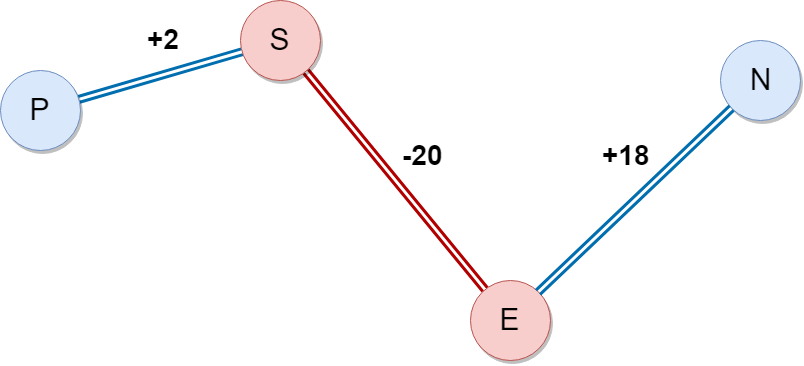
\includegraphics[width=\textwidth]{Fotos/np_mutation/Case1.png}
	\caption{Case where note E is going to be transposed upwards.}
	\label{fig:npmut_case1}
\end{figure}

The next case is illustrated at figure \ref{fig:npmut_case2}. The absolute value of the next semitone is higher than the previous one just like the previous case, but the direction of the middle interval, however, is not different than the next interval. We now have chosen to transpose the start note downwards in the algorithm.

\begin{figure}[H]
	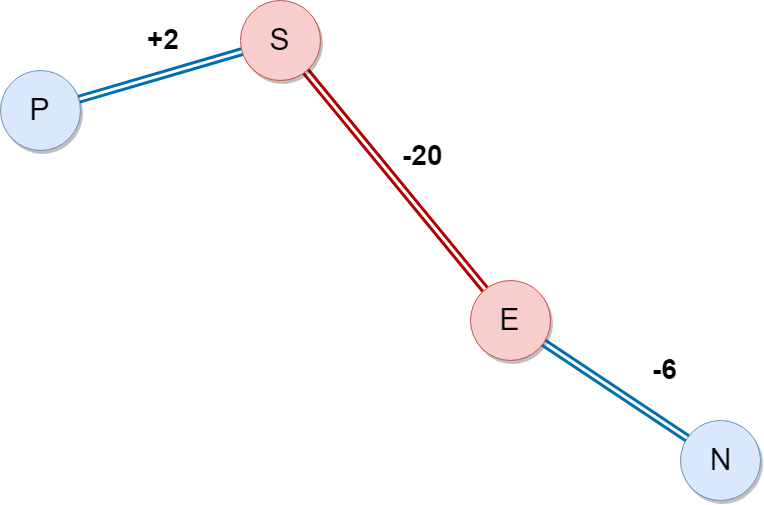
\includegraphics[width=\textwidth]{Fotos/np_mutation/Case2.png}
	\caption{Case where note S is going to be transposed downwards.}
	\label{fig:npmut_case2}
\end{figure}
The two cases that are left have similar behaviour but in an opposing manner. Here, the absolute value of the next semitone is lower than the previous one just like the previous cases. We now determine which note to select by comparing the previous interval direction with the middle one instead of comparing the middle interval direction with the next interval direction. If the direction of the middle and previous interval are the same the end note E is selected, else the start note S.


\paragraph{Transposing and correcting the selected note}\mbox{}\\
Now that we have determined which note to transform, there are only two things left to arrange: transposing the note and correcting it according to the song's scale. On listing \ref{code:transposing_the_note} a simplified version of the algorithm for transposing and correcting the note has been listed. 

\begin{lstlisting}[language=Python,caption={Part 3 of the simplified version of the Neighbour pitch mutation algorithm: transposing and correcting the note.},captionpos=b,label=code:transposing_the_note]
#PART3 Transposing the note

#Selecting the direction of the transposition
if selected_note == middle_interval.noteStart:
	sign_multiplier  = 1
else:
	sign_multiplier  = -1

aInterval = interval.Interval(
				sign_multiplier * 
				round(middle_semitone*self.pitch_action_strength)
				)
				
#Transpose the note
selected_note.transpose(aInterval,inPlace = True)

#Correcting the note according to the scale
scale = song.scale
pitch = random.choice(scale.pitches) #choosing random pitch from scale
name = pitch.name + str(noteA.octave)
noteB = note.Note(name)

ainterval = interval.Interval(noteStart=selected_note, noteEnd=noteB)
semitone = ainterval.semitones

#If there is a note that is closer than its current octave
if abs(semitone) > 7:
	if semitone > 0:
		semitone -= 12
		temp = interval.Interval(-12)
	else:
		semitone += 12
		temp = interval.Interval(12)

noteB.transpose(temp, inPlace=True)
ainterval = interval.Interval(noteStart=noteA, noteEnd=noteB)

object.transpose(value=interval.Interval(semitone), inPlace=True)

\end{lstlisting}

First, we determine the direction that the note is supposed to transpose. If the start note is selected, we transpose it with the direction of the middle interval. The result makes the middle interval smaller, what exactly is the point is of this whole mutation. If the end note is selected, we need to transpose it in the opposite direction of the middle interval in order to make the interval size smaller.
\\\\
Now that we know which direction we are going, we determine the strength. This strength is based on the size of the middle intervals semitone. The variable $pitch\_action\_strength$ is a ratio between 1 and 0 that determines the strength of the pitch mutation. This is set to $0.5$ by default. The higher this variable, the stronger the mutation will be.
\\\\
After the transposition, we correct the note according to the scale of the song so it fits well enough in the bigger picture. We randomly select a pitch from the scale and then create a note with this pitch within the same octave as the selected note (the note we reached by previously transposing). This new note, the scale correct note, is supposed to be the note that is the closest to the selected note with its pitch randomly selected from the song's scale. Finally, we transpose the selected note to this scale correct note. Notice that this will also affect the scale correctness sub rater, section \ref{subrater:scale_corr}, when we transform an out of scale note into a scale correct note. 
\\\\
We now successfully made a wrong interval less wrong by decreasing the interval size.


\subsubsection{Measure swap mutation}
This mutation selects two measures in a random or planned way and swaps their place in the song. The selection happens in an interesting way. Let us call the measures that we are about to swap with each other measure A and measure B. The selection of measure A will be random or planned by a chance rate of 50\%. So half the time the selection of A is random the other half it is somewhat logical.
\\\\
When the selection is random, there is no explanation necessary. When it happens logically, however, some explanation would be useful. In the section \ref{sec:relmeasurebasedratings} we discussed sub-raters based on the distance of the master by calculating measure per measure and adding them up. When we calculated each measure's rating, we stored this rating in the measure so we can use it at this point of the application. Measure A is chosen based on this value: we chose the worst-rated measure.
\\\\
Measure B is always chosen randomly and measure B must not be equal to measure A. After having correctly chosen the measures, we swap them. The reason for a measure swap is to manipulate the ratings that are based on the measures. We do want to add some randomness to the order the measures in songs occur in and the resemblance of the measures.

\subsubsection{Measure mix mutation}
This mutation selects two measures A an B the same way as the measure swap mutation. After selection, we take some elements of measure B and put them inside of A. This way we actually put random elements from another measure into measure A that is likely to be a bad measure (50\% at the time).


\subsubsection{Element swap mutation}
This mutation is self-evident, we take two random elements from the song and simply swap them. Just like the measure swap mutation, the purpose of this mutation is to play with the order of elements in the song.

\subsubsection{Element type mutation}
We take an element (rest, note or chord) out of the song and replace it with another already existing element in the song that has a different type. The duration of the note will be unchanged. This mutation has a direct effect on all the sub-ratings that are based on the types of the song.

\subsubsection{Element pitch mutation}
This mutation takes a random chord or note out of the song and transposes it within the limits. These limits are determined by the theory or the master song. This limit is the same as the limit that defines a wrong interval (more about this in section \ref{sec:rater:neighbourpitch}). We need to stay in-between these limits in order to prevent messing up the neighbour pitch rating.


\section{Results}
\subsection{Domain and input parameters}
In order to calculate the results and we needed to define a domain where we are going to execute the program. We experimented with the constants and values to achieve the best result. 
\subsubsection{Global parameters}
First up, the most interesting and deeper results we got from the sub-rating system with a master song. This way we were able to use all the sub-ratings that can only be used when there is a master song. That way we can try to recognize patterns between our output songs and the master song.
\\\\
Second, we need to define the number of measures and the number of parents. We noticed the following results. The larger the number of parents, the lower the impact a bad mutation would have on the best rated next child, but the longer it takes to generate a generation. Thus we needed to find a value in-between. We were looking for a value n, where it should not take too long to produce a generation and a mutation would mess up the total rating of the next fittest song. 
\\\\
Let us first explain why a bad mutation would result in a negative score when we lower the number of parents. The number of parents, P, is a representation of how many songs will be selected for the next generation. When it comes to mutation, we are at the state where we just selected the P fittest children. These children, the rated children, now will have a chance to be mutated positively or negatively. We only mutate a fraction of the songs. One bad mutation on a song out of four songs will have a much bigger impact on one bad mutation on a song out of 8 songs. The chance that a bad mutation will be taken with the crossover function is less when we have more parents we are going to pair the badly mutated song with. We had the following results illustrated on the chart on figure \ref{fig:parents_time}:

\begin{figure}[H]
	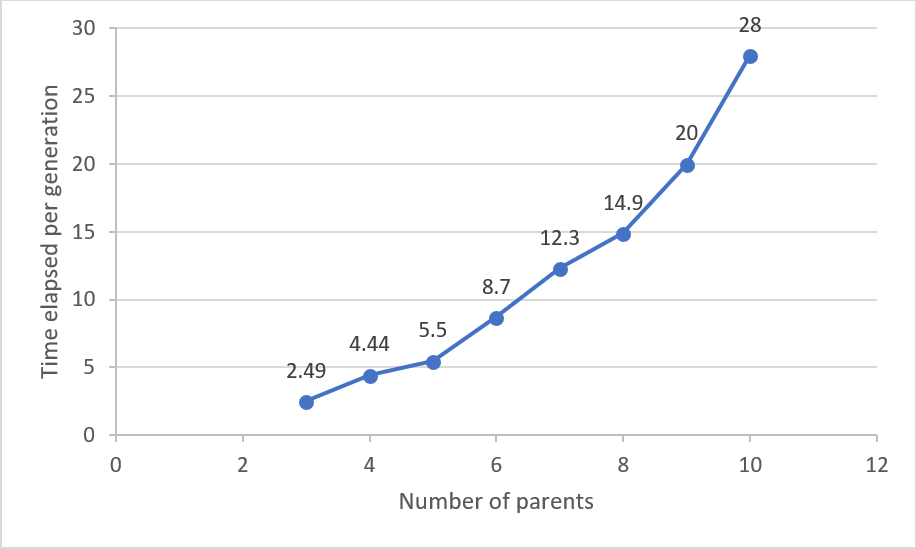
\includegraphics[width=\textwidth]{Fotos/parents_time_graph.png}
	\caption{Chart of number of parents over time per generation.}
	\label{fig:parents_time}
\end{figure}

We determined that somewhere around 6 and 8 is justifiable. Here, it nor took too long for a generation, neither did a bad mutation impact the score in a significant way. Just assume we have 7 parents for now.
\\\\
The number of measures is important for the speed of execution: the longer a song, the more elements need to be considered crossing with each other, the more elements and measures need to be rated. We need a considerable amount of measures that has enough place for multiple repetitions over the song. If a song only has four measures, multiple repetition is very difficult. That is why we came up with a song that has four times four measures, meaning 16 measures. This amount is enough to have repetition variations and will have a fast enough execution rate.
\\\\
At last, we have two more parameters left: the number of generations and the master song. The number of generations usually depends on what we are or trying to achieve. The more generations we have the better our results will be, the longer it will take. Luckily we tend to write every generation as a file so we can check the songs during execution. We do not have to wait until we have reached our last generation.
\\\\
The master song is just a string with the path of the song that should be considered to be the master.

\subsubsection{Rating weights and parameters}
As mentioned in section \ref{sec:rating}, every sub-rater has a weight where the calculated score will be multiplied with. We are allowed to play with these weights to focus on different concepts of a song. On listing \ref{code:weights_1} we have put a commonly used setting for the weights and parameters.

\begin{lstlisting}[language=Python,caption={Weights and parameters of for the sub-raters.},captionpos=b,label=code:weights_1]
# region IntervalRater
# WEIGHTS
NEIGHBORING_PITCH_WEIGHT = 10
MELODY_DIRECTION_WEIGHT = 1
DIRECTION_STABILITY_WEIGHT = 1
UNIQUE_PITCHES_WEIGHT = 1
# DEFAULTS
MAX_INTERVAL_SIZE = 20
MIN_INTERVAL_SIZE = -20
MELODY_DIRECTION = 0.5
DIRECTION_STABILITY = 0.5
UNIQUE_PITCHES_RATE = 0.5
# endregion

# region RepetitionRater
# WEIGHTS
MEASURES_RATING_WEIGHT = 25
BINDINGS_RATING_WEIGHT = 25
# DEFAULTS
MASTER_STRONG_MEASURES_RATIO=0.5
MASTER_NORMAL_MEASURES_RATIO=0.3
MASTER_WEAK_MEASURES_RATIO=0.2
MASTER_GARBAGE_MEASURES_RATIO=0.2
MASTER_STRONG_BINDINGS_RATIO=0.5
MASTER_NORMAL_BINDINGS_RATIO=0.3
MASTER_WEAK_BINDINGS_RATIO=0.2
MASTER_GARBAGE_BINDINGS_RATIO=0.2
#endregion

# region SampleBasedRelativeMeasureRater
# WEIGHTS
TYPES_DISTANCE_RATING_WEIGHT = 10
SEMITONES_DISTANCE_RATING_WEIGHT = 10
PITCHES_DISTANCE_RATING_WEIGHT = 10
DURATION_DISTANCE_RATING_WEIGHT = 10
OFFSETS_DISTANCE_RATING_WEIGHT = 10
# endregion

#region MusicalRater
#WEIGHTS
SCALE_CORRECTNESS_WEIGHT = 2
ZIPFS_LAW_DISTANCE_PITCHES_WEIGHT = 0
ZIPFS_LAW_DISTANCE_INTERVALS_WEIGHT = 0
#DEFAULTS
SCALE_CORRECTNESS_RATING = 0
ZIPFS_LAW_DISTANCE_PITCHES = 0
ZIPFS_LAW_DISTANCE_INTERVALS = 0
#endregion

# region SampleBasedAbsoluteRaterStrategy
# WEIGHTS
ABSOLUTE_RHYTHM_WEIGHT = 10
ABSOLUTE_TYPES_WEIGHT = 10
INTERVAL_DISTR_DISTNCE_RATING_WEIGHT = 10
TYPES_DISTR_RATING_WEIGHT = 7
ELEMENT_COUNT_WEIGHT = 10
#endregion

\end{lstlisting}

Notice that the weights in $SampleBasedMeasureRater$ and $SampleBasedMeasureRater$ are much higher than the others. This is a result of the size of the values. The scores of these ratings are significantly small. Remember that these scores are calculated based on a maximum Wasserstein distance, this maximum distance is relatively very large. This results in the scores being relatively very low value. Therefore the multiplying weight must be higher than usual in order that the rating will have an effect on the total rating.

\subsubsection{Mutation parameters}
During the mutation process, there are some parameters that define the way songs are mutated. In section \ref{sec:mutation} we brought up various elements like probabilities and differences between the fittest and the least fit child.
\\\\
We used the following two parameters: the likelihood that a song will be chosen to be mutated, $mutation\_probability$, is 40\% and the likelihood that a song will be chosen for re-mutation, $remutation\_probability$, is 10\%.
\\\\
On listing \ref{code:mutation_probabilities} we have put the code where it is clear in which order the mutations happen to be and with what probabilities.

\begin{lstlisting}[language=Python,caption={individual mutation probabilities.},captionpos=b,label=code:mutation_probabilities]
choice = random.random()
if choice < mutation_probability:
self.pitch_mutation(song)

choice = random.random()
if choice < mutation_probability/2:
self.swap_measure(song)

choice = random.random()
if choice < mutation_probability/2:
self.mix_measure(song)

choice = random.random()
if choice < mutation_probability:
self.swap_notes(song)

choice = random.random()
if choice < mutation_probability:
self.mutate_type(song)

choice = random.random()
if choice < mutation_probability:
self.mutate_duration(song)

choice = random.random()
if choice < mutation_probability:
self.mutate_pitch(song)

choice = random.random()
if choice < remutation_probability:
self.mutate(song)

\end{lstlisting}

As you can see the mutation associated with the measures, measure swap and measure mix, have a lower probability. These mutations mess up with the size of the song. It is a known technical difficulty, however, we noticed that when these mutations tend to happen fewer, problems do not occur.
 


\subsection{Results of the executions}
In this section we describe executions and the result we had from them.
\subsubsection{RHCP - Californication 16 measures 7-10 parents}
This song has a very high repetition rate, the first two measures are almost repeated over the whole song. We expect a recognizable repetition in the end results. We know this song does not have crazy interval jumps and is genuinely filled with notes for the most part. 

We used the following songs for the initial population:
\begin{itemize}
	\item Portal 2 - Cara Mia
	\item Godfather theme song
	\item Debussy - Clair de Lune
	\item Chopin Mazurka, Op. 7 No. 1
	\item Queen - Bohemian Rhapsody 
	\item Beethoven Op.10 No.1 
\end{itemize}

First, we added more note swaps and lowered the measure mutations. What we ended up doing was that a song could have four note swaps at a single mutation and the chances of measure mutation have been lowered by 50\%. On figure \ref{fig:rhcp_1} we plotted the total rating against the generation number. We can see that after the first 60 generations, the ratings do not change that much. The score tends to get lower with time, which is a good thing, but it takes too long. 

\begin{figure}[H]
	\advance\leftskip-1.5cm
	\includegraphics[width=1.2\textwidth]{Fotos/results/rhcp/total_rating_graph.png}
	\caption{Chart for total rating with: master song Californication, 16 measures, 7 children, very low measure mutation rates, 144 generations.}
	\label{fig:rhcp_1}
\end{figure}

The reason for this is that the ratings based on the measures are not affected that much because of the low rates of the measure mutation. We can clearly see it on figure \ref{fig:rhcp_1_m}. These sub-raters shown on the graph are based on the measures. After a while, they stabilize and do not tend to change much.


\begin{figure}[H]
	\advance\leftskip-1.5cm
	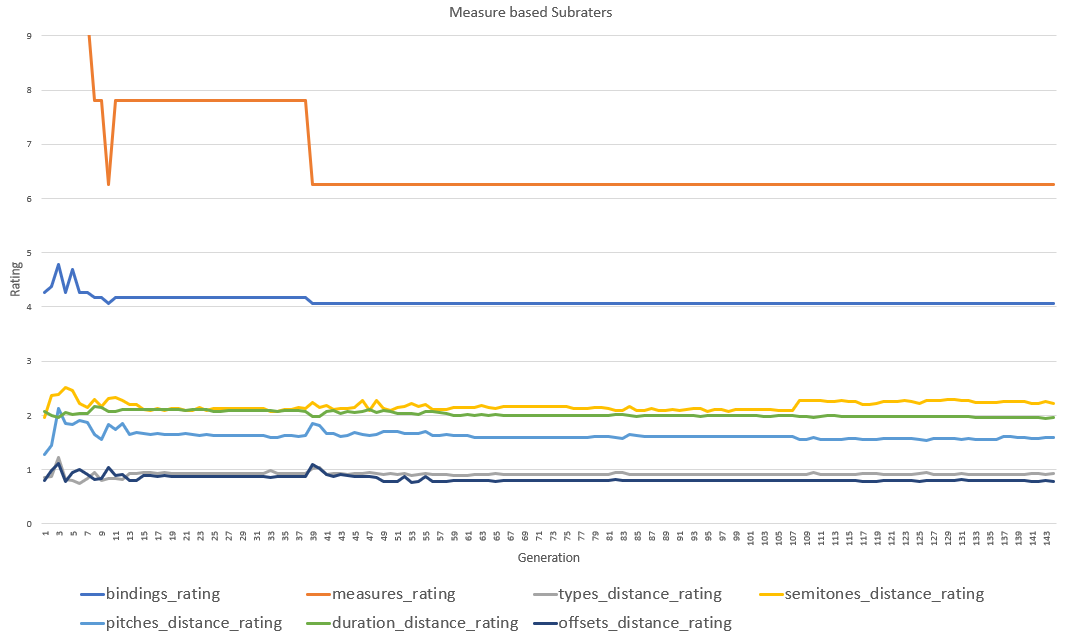
\includegraphics[width=1.2\textwidth]{Fotos/results/rhcp/measures_rating.png}
	\caption{Chart for measures based sub-raters: master song Californication, 16 measures, 7 children, very low measure mutation rates, 144 generations.}
	\label{fig:rhcp_1_m}
\end{figure}

We like to put the probabilities for measure mutators higher and go on with the children of the last generation we just created. After 140 generations with a higher probability of mutation of measures, we get the same results. Yes, it is more likely to get the measures ratings a little lower, but certainly not low enough. We want to hear some repetition in the final generation's fittest song. All we can hear right now is that the measures tend to use the same notes and chords and do have some kind resemblance with each other. We are searching for absolute recognizable resemblances of measures that repeat each other.
\\\\
We tried doubling the sub-rater's weights wishing that positive impact in measures would affect the total rating stronger than it used to do. We also removed the measure mix mutation because it seems it affects the score in a negative way. After 167 generations we saw that the results got a little better. There still needs to be a better way of dealing with this.
\\\\
Instead of only playing with the weights we tried to play with the number of parents and the mutation probabilities in general. We know that we already have some kind of a stable population that will not change much with the crossover process not to forget that the parents do not differ that much from each other. The only way to introduce possible improvements is through the mutations. The mutation probability is now set to 60\% instead of 40\%. The number of parents is raised by two so we got 8 parents. 
\\\\
In short, more mutations and more children to choose from. We also play with some weight. The relative based measure sub-ratings weight will be doubled. These sub-ratings are explained in detail in section \ref{sec:relratings}. The bindings ratings and the measure weight that we earlier doubled will be set to their normal value. The results we gained from these settings are still not what we were searching for. We need to keep looking for a better configuration that will lead us in the right direction.
\\\\
After a number of experiments with weights, mutations and number of parents, we have achieved what we were looking for. What we did was the following: we lowered the maximum population difference value to 5\%. This value is explained in section \ref{sec:mutation}, what this means is that mutations will happen when the songs of the population are more similar to each other. We set the barrier higher for entering mutation. This means that the songs have become more alike before mutating them. Mutations will cause dissimilarities in songs and what we did is letting the crossover, rating and selection process deal with these dissimilarities. After a while, the songs will get similar to each other and all the bad mutations will have a chance to work themselves out and the good ones to stay for the most part. When the population is ready (meaning similar to each other) we can mutate them. This mutation will most likely make the population dissimilar again. We are forcing changes to happen.
\\\\
Furthermore, we set the number of parents to 10 meaning we have 45 children after crossing them with each other. By incrementing the number of children we got more possible outcomes to choose from thus bad mutations are less likely to survive because there are more children to choose from. A badly mutated song will pair with more songs as it did before, but the crossover process is random meaning the part where the bad mutation takes place will not always be chosen in the paired song. More songs mean that the probability that every time the bad part has been ended up in the paired song will become less likely. Let us illustrate this with the following example. Consider the classic example where we flip a coin, heads is where the bad mutation occurs in the paired song and tails where it does not. We would want to have as many possible coin-flip results to choose from as possible. For example, if we only do two coin-flips the chance that the results would be all heads is higher than if we did 10 coin-flips.
\\\\
We also changed some weights here and there: we concentrated on the $SampleBasedMeasureRater$ weights by increasing their value. We also lowered the $NEIGHBORING\_PITCH\_WEIGHT$ from $10$ to $1$ because some mutations would create a negative effect on this neighbour pitch rating. Since the neighbour pitch mutation deals with these wrong intervals, they will eventually be eliminated.
\\\\
At last, we changed some probabilities in the mutation process and even changed a mutation itself. We created a new probability that is only responsible for the number of songs that are going to be mutated: $song mutation probability$. This value is set to 80\%. This allows us to mutate more songs of the population. When a song is chosen for mutation it still needs to face another probability per mutation: $the mutation probability$. This is the probability that every mutation needs to face, as it was shown on listing \ref{code:mutation_probabilities}. This value is set to 0.4. We can sum this up as follows: we increased the number of songs that are selected for mutation while keeping a relatively low amount of mutations on them. The mutation we changed is the measure mix. Instead of adding elements from one measure to another we completely removed the measure and copied another one as its replacement. We believe this will have a positive effect on the repetition of the song and it successfully did.

\begin{figure}[H]
	\advance\leftskip-1.5cm
	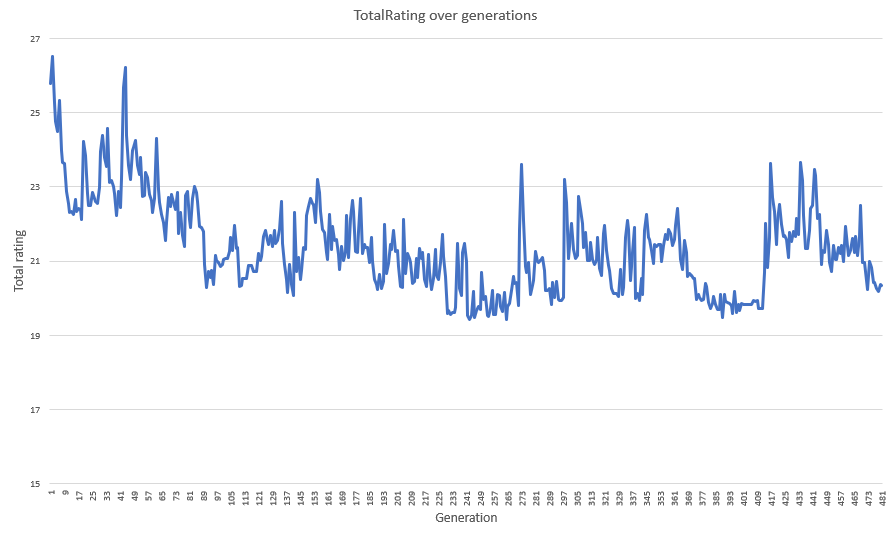
\includegraphics[width=1.2\textwidth]{Fotos/results/rhcp/total_rating_2_graph.png}
	\caption{Chart for total rating with: master song Californication, 16 measures, 10 children, very high measure mutation rates, 481 generations.}
	\label{fig:rhcp_2}
\end{figure}

On figure \ref{fig:rhcp_2} we see the same improvement as we did before but this time we have 481 generations instead of 144. As you can see on the chart there are a lot of fluctuations, this is because we used a lot of mutations. The big question is what happened to repetition ratings, did we create more repetition as we did before? When we Listen to the last generation's song, we clearly hear that there is indeed some repetition.

\begin{figure}[H]
	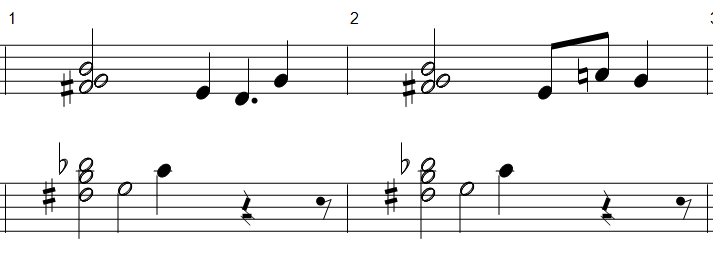
\includegraphics[width=\textwidth]{Fotos/results/rhcp/song2.png}
	\caption{First two measures of the fittest song from generation 481.}
	\label{fig:rhcp_2_song}
\end{figure}

The two measures shown on figure \ref{fig:rhcp_2_song} do repeat themselves at other parts of the song. Most elements of these two measures are repeated over and over in 7 out of 16 measures. The other measures have some parts of these measures in common alongside their own unique parts. This means we are getting closer achieving the repetition level of the master song.


\begin{figure}[H]
	\advance\leftskip-1.5cm
	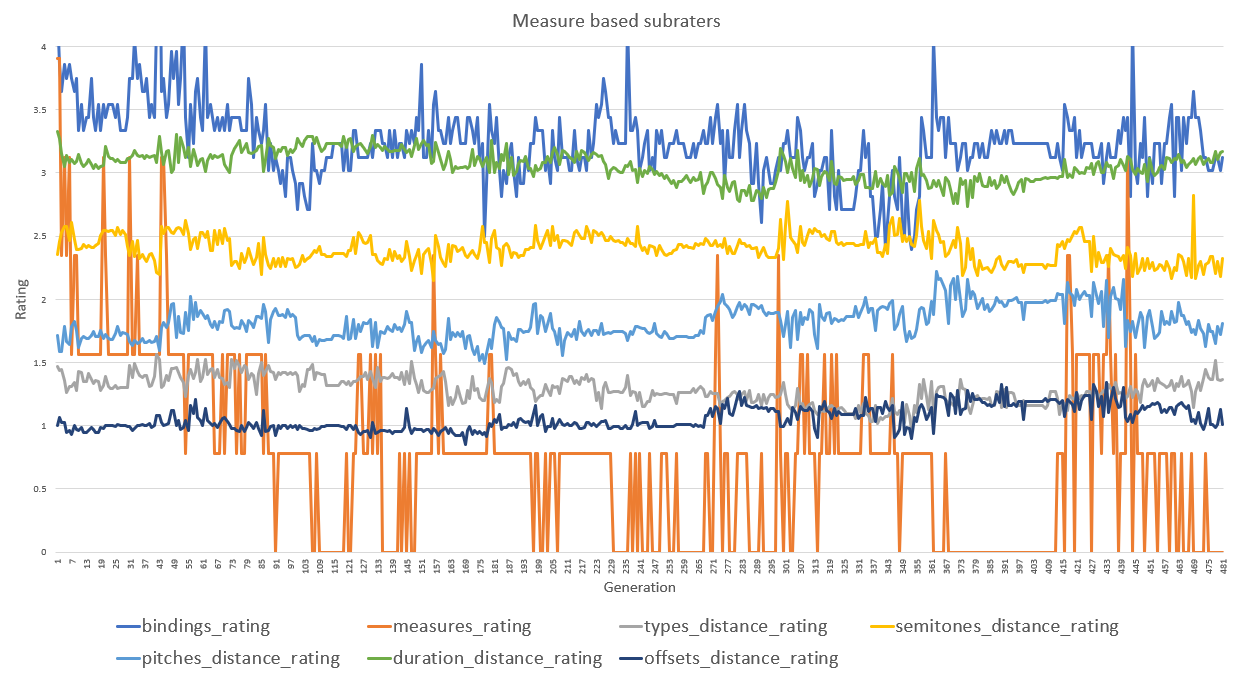
\includegraphics[width=1.2\textwidth]{Fotos/results/rhcp/measures_rating_2.png}
	\caption{Graph for measures based sub-raters: master song Californication, 16 measures, 10 children, very high measure mutation rates, 481 generations.}
	\label{fig:rhcp_2_m}
\end{figure}

There is a lot going on figure \ref{fig:rhcp_2_m}, almost all the ratings hang around the same area, except for the measure rating. This measure rating goes at multiple points to 0 meaning the measures type distribution is exactly the same as the master song's (more about the measures type distribution in section \ref{sec:measure_type}). That is why we hear a lot of measures that are much like each other. Notice that the bindings rate also has a drop-down from larger than 4 to somewhere around 3. This may look like it will have little impact, but little changes in this value mean a lot in reality. The reason for this is that this value is calculated based on the huge maximum distance as explained earlier. Little value values based on large values will have a minor impact on the final score.
\\\\
Let us take this procedure to the next level: take the latest population and start generating further with this time 9 parents and 2615 generations on top of the previous 481. 


\begin{figure}[H]
	\advance\leftskip-1.5cm
	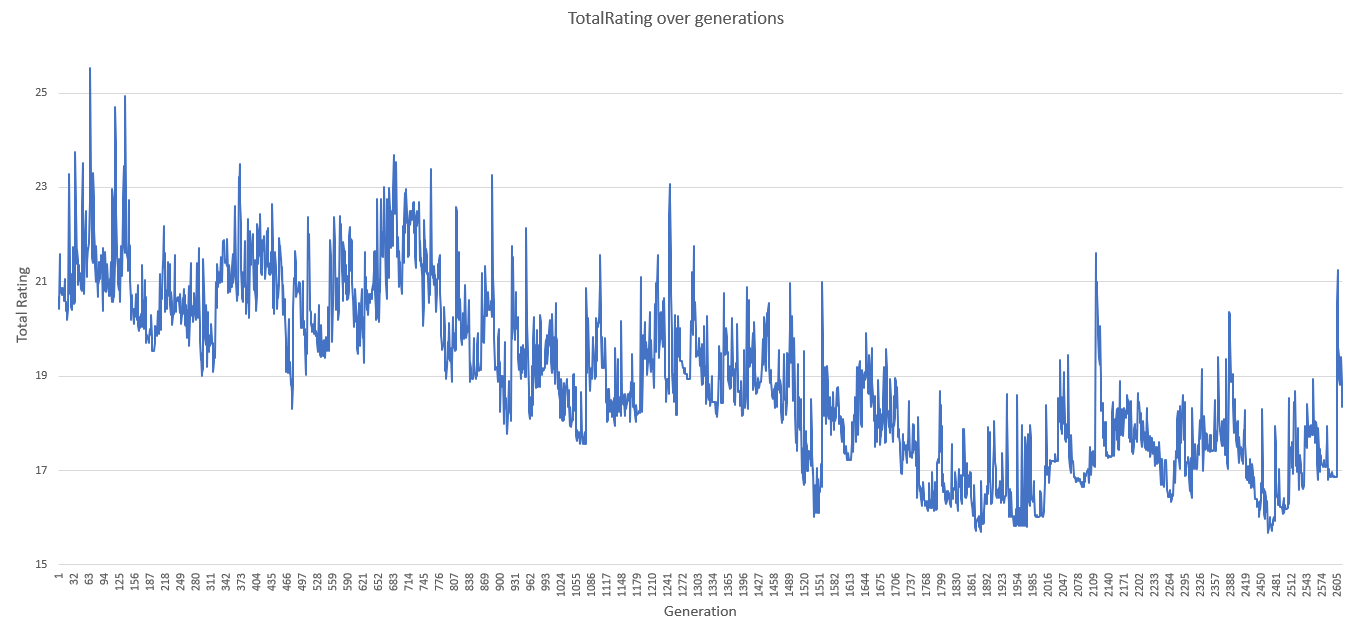
\includegraphics[width=1.2\textwidth]{Fotos/results/rhcp/total_rating_3_graph.png}
	\caption{Graph for total rating with: master song Californication, 16 measures, 10 children, very low measure mutation rates, 2615 generations.}
	\label{fig:rhcp_3}
\end{figure}

On figure \ref{fig:rhcp_3_m} the measure based ratings are plotted on a chart. We clearly see that the ratings go up and down around a fixed position, however, the bindings rating lowers itself from around 3.5 to 1.2. This has a significant impact on the resulting population. This also explains the high level of repetition in the fittest song of the last generation. Even though it being not easy to recognize repetition on figure \ref{fig:rhcp_3_song}, you can clearly hear it when listening to the song. For example measures, 3, 5 and 7 have massive similarities. The measures 2,4 and 6 have the same elements on their first half.

\begin{figure}[H]
	\advance\leftskip-1.5cm
	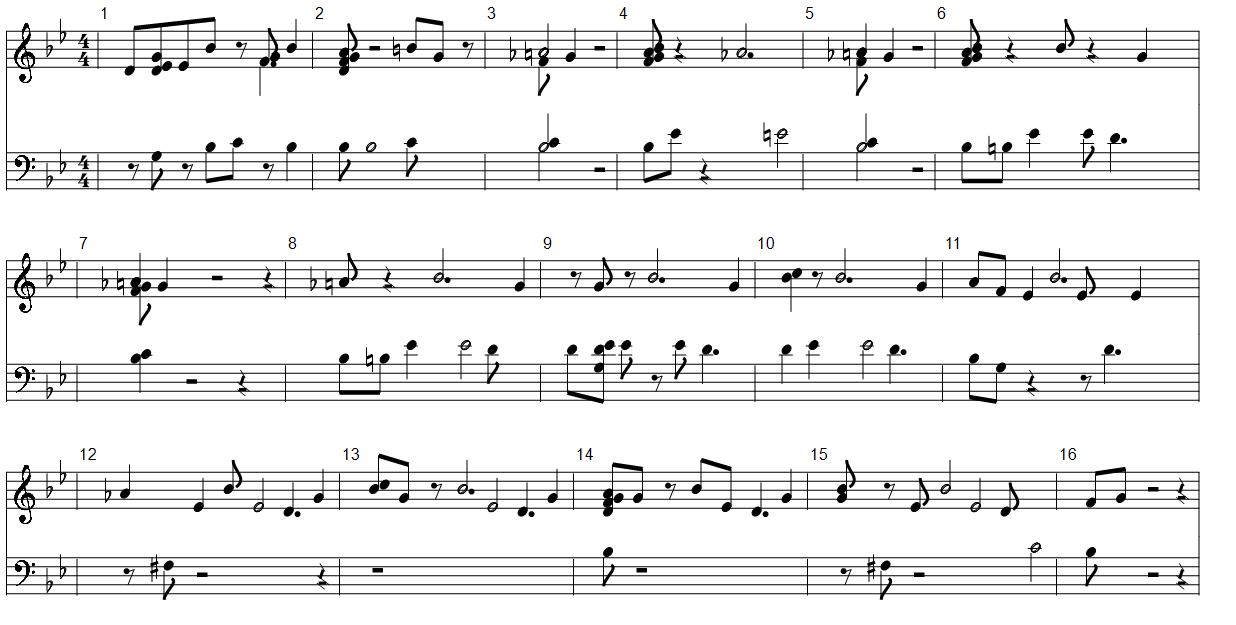
\includegraphics[width=1.2\textwidth]{Fotos/results/rhcp/song3.png}
	\caption{The fittest song from generation 2615.}
	\label{fig:rhcp_3_song}
\end{figure}

\begin{sidewaysfigure}[ht]
	\advance\leftskip-1.5cm
	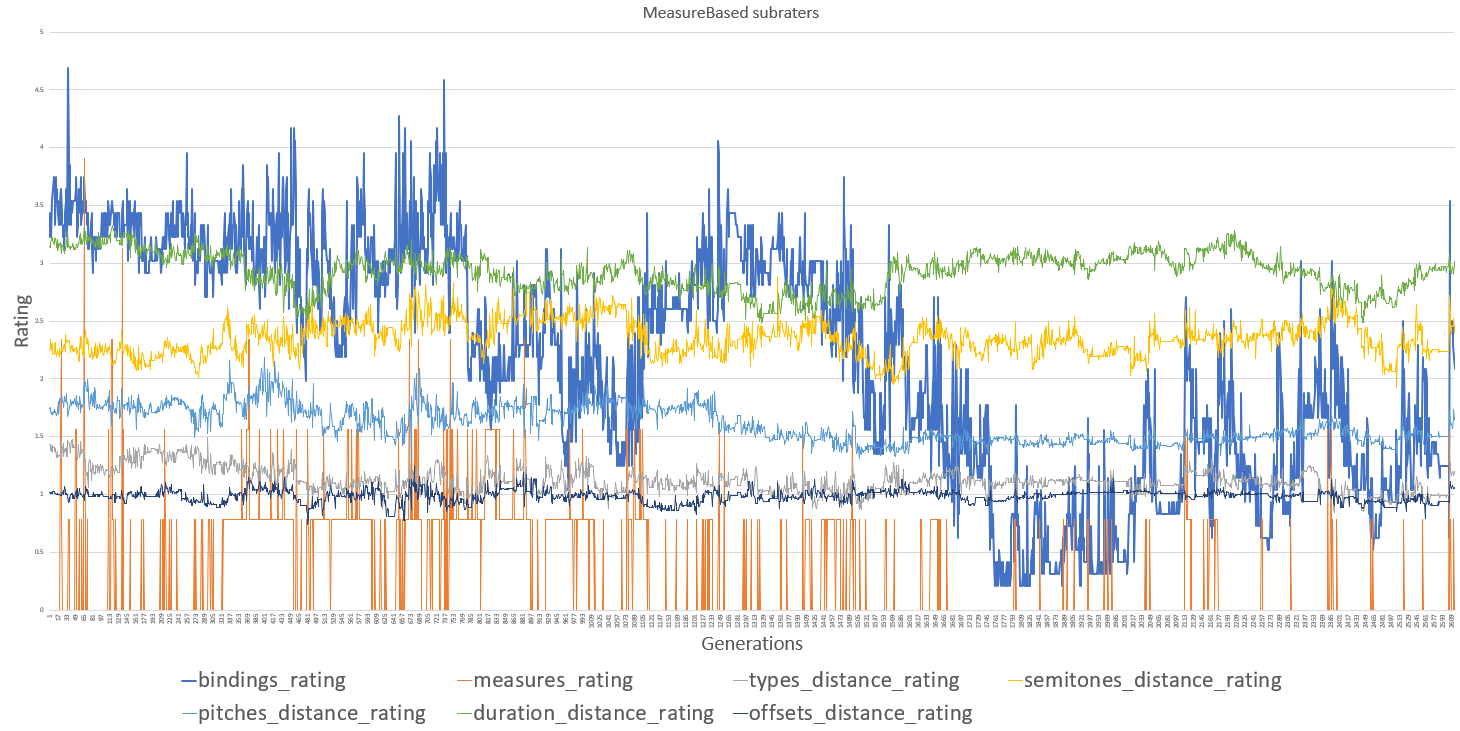
\includegraphics[width=1.2\textwidth]{Fotos/results/rhcp/measures_rating_3.png}
	\caption{Graph for measures based sub-raters: master song Californication, 16 measures, 10 children, very low measure mutation rates, 2615 generations.}
	\label{fig:rhcp_3_m}
\end{sidewaysfigure}

\clearpage


\paragraph{Final thoughts}\mbox{}\\
If we look at the results, we can clearly see that the stream of notes is like the master song. The interval's behaviour does match the master. The type distribution is looking good. In the first 300 generations, we can recognize the elements from the initial population but that slowly fade away which is self-evident. More generations and parents will result in better results, especially when we have a lot of mutations.



\subsubsection{The Godfather theme song - 16 measures 9 parents}

We used the following songs for the initial population:
\begin{itemize}
	\item Portal 2 - Cara Mia
	\item rhcp - Californication 
	\item Debussy - Clair de Lune
	\item Chopin Mazurka, Op. 7 No. 1
	\item Queen - Bohemian Rhapsody 
	\item Beethoven Op.10 No.1 
\end{itemize}

This song has some repetition but unlike the previous master song, Californication, there are various measures that repeat instead of only 2. We bring up the graph that represents the strong measure and their bindings from section \ref{sec:measure_rel}, displayed again on figure \ref{fig:GF_strong_graph2}.

\begin{figure}[H]
	\includegraphics[width=\textwidth]{Fotos/bindings_graph/Godfather_16_strong.png}
	\caption{Graph representing strong bindings between measures of the Godfather theme song: 9 nodes, 6 bindings. Each node is a measure with its number inside, each edge represents the strength of matching rate between them.}
	\label{fig:GF_strong_graph2}
\end{figure}

Now that we have taken a step backward from repetition we'll find us stranded on a more complex space: making music sound good with less repetition. We previously learned that we need a lot of generations until we get something to work with and that mutations can work in our favor over a long extended period of time with at least 500 generations. Also having more parents will result in successful progress. We changed our strategy a little based on the previous results.
\\\\
First, the probability for mutating a song is set to 70\%. This is mainly because we want to prevent mutating in many songs. We saw on the previous results that during the generations there were moments where the rating significantly increased. We want to prevent this from happening. Next up we decreased the mutation probability to 20\% instead of 40\%, this is the one that is listed on listing \ref{code:mutation_probabilities}. The same reason applies here: making sure we decrease the rating value in a stable way. We want to prevent upstrokes in the ratings as much as possible. We chose to have 16 measures and 9 parents. We ended up with 2960 generations. Figure \ref{fig:gf_1} shows the results of the total ratings of all generations.

\begin{figure}[H]
	\advance\leftskip-1.5cm
	\includegraphics[width=1.2\textwidth]{Fotos/results/gf/total_rating_graph.png}
	\caption{Graph for total rating with: master song the Godfather theme, 16 measures, 9 children, very low measure mutation rates, 2960 generations.}
	\label{fig:gf_1}
\end{figure}

We can still see a lot of fluctuations. We noticed that the further the generation, the harder it is to get a lower value than the previous one. The strength of the rating's decrease will go down whenever the generation number goes up. This means it is harder to make a song better when it has already been made better previously.
\\\\
Let us break down the total rating's chart down to the separate categories to analyze their rating variations during the evolution from the start to the end.
\\\\
First, let us talk about music theory. On figure \ref{fig:gf_musical} a chart has been plotted with the three theory-based raters: Scale correctness, Zipf's law on pitches and Zipf's law on intervals. These ratings vary a lot but around their fixed point. They start high and immediately after say 30 generations they decrease themselves only to stay around their fixed point. We see that both Zipf's law on pitches and Zipf's law on intervals sub-ratings come close to perfect which is a good sign. The scale correctness rating, however, goes a little upwards. This is mainly because of the mutations and other sub-ratings interfering with its success. If a mutation benefits another sub-rating and disadvantages another, the application will listen to the one with eventually the most impact (probably has the highest weight). We can conclude this out of the fact that the total rating is going down.

\begin{figure}[H]
	\advance\leftskip-1.5cm
	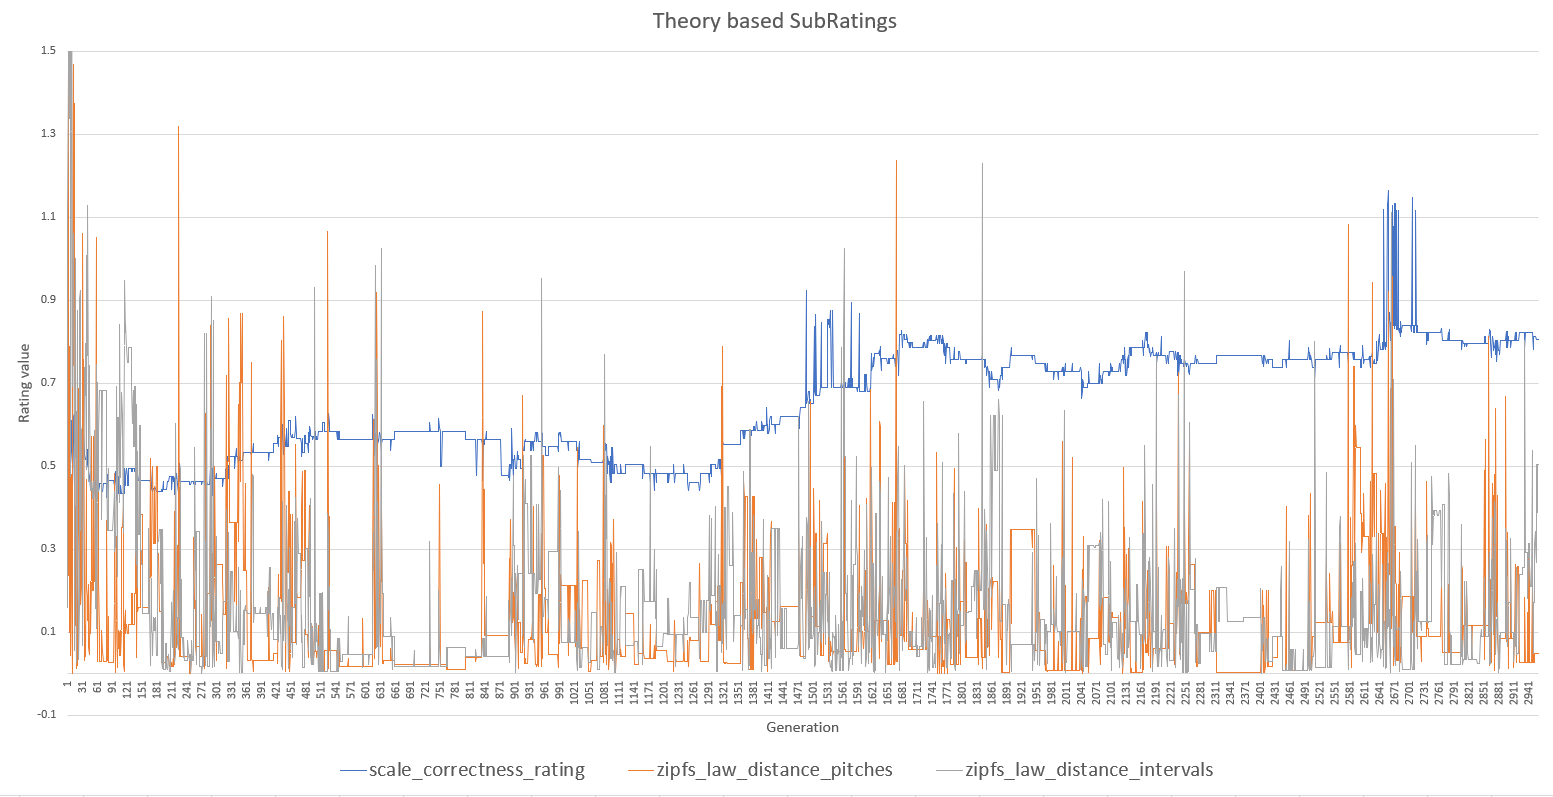
\includegraphics[width=1.2\textwidth]{Fotos/results/gf/musical_rating_graph.png}
	\caption{Chart represents the music theory sub-ratings over generations.}
	\label{fig:gf_musical}
\end{figure}

Next up we have the intervals and pitches sub-ratings (figure \ref{fig:gf_interval}). These sub-ratings try to make sure the melody is in the norms of the one characterized in the master. All of these sub-ratings successfully manage to lower their value over the generations through. They start getting better fast and do not really stop getting better until they hit the bottom. These sub-raters also fluctuate around a fixed point.

\begin{figure}[H]
	\advance\leftskip-1.5cm
	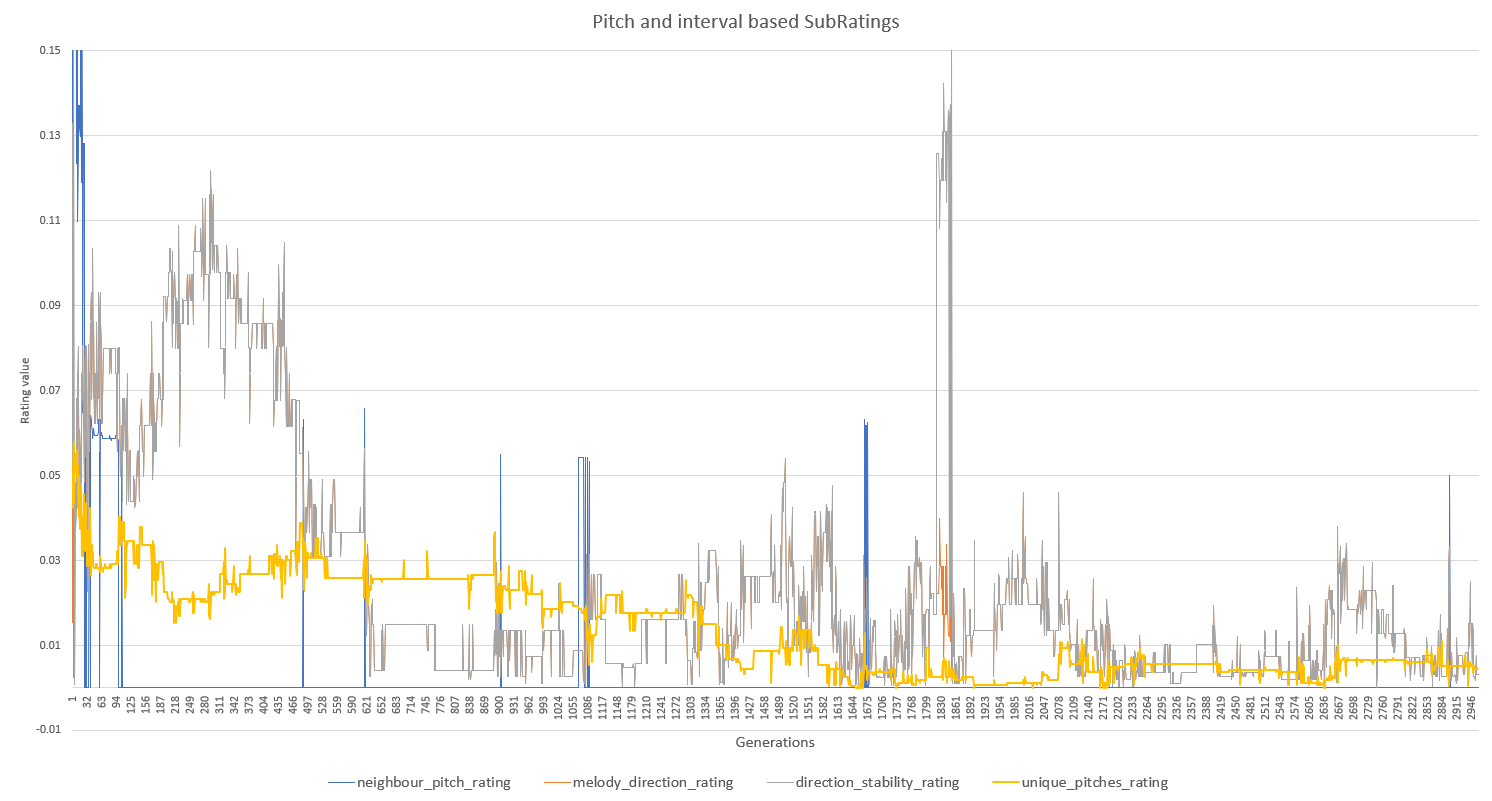
\includegraphics[width=1.2\textwidth]{Fotos/results/gf/interval_rating_graph.png}
	\caption{Chart represents the intervals and pitches sub-raters over generations.}
	\label{fig:gf_interval}
\end{figure}

On figure \ref{fig:gf_measures} a chart is plotted with two measures distribution ratings: bindings and measure ratings (section \ref{sec:measure_rel}). For the measure distribution, we hit the bottom very fast. The bindings rating, however, takes some time until reaching perfection. The genetic algorithmic process successfully satisfies these sub-raters.

\begin{figure}[H]
	\advance\leftskip-1.5cm
	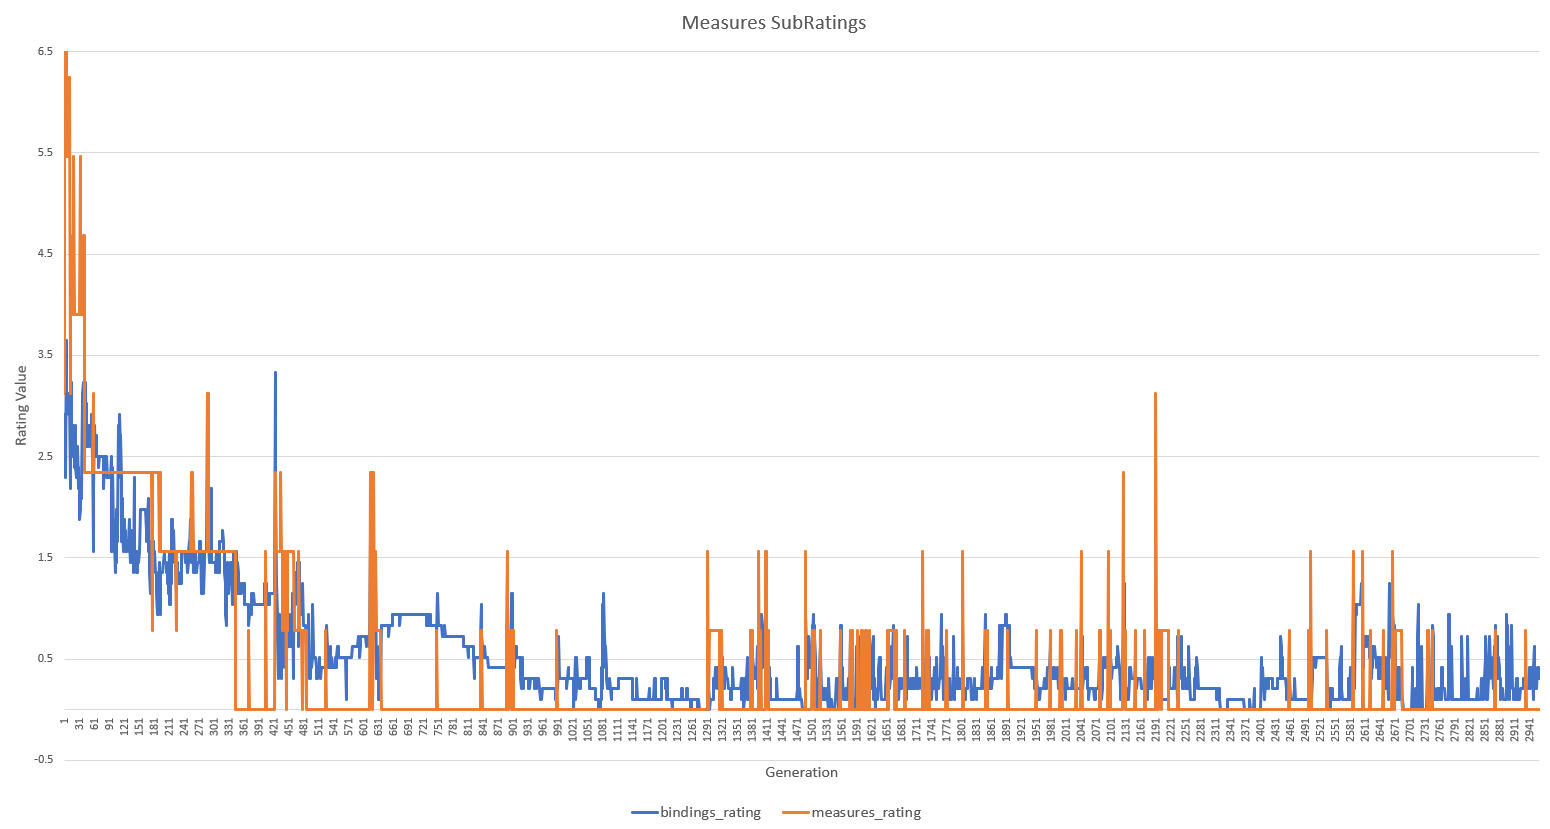
\includegraphics[width=1.2\textwidth]{Fotos/results/gf/measures_rating_graph.png}
	\caption{Chart represents the measure distribution sub-raters over generations.}
	\label{fig:gf_measures}
\end{figure}

The relative measure sub-raters have a difficult time getting better. As it is visible on the chart on figure \ref{fig:gf_relm}, the raters only are able to lower themselves on the initial start. This means that it is harder for those values to get better based on the mutation processes we provide.


\begin{figure}[H]
	\advance\leftskip-1.5cm
	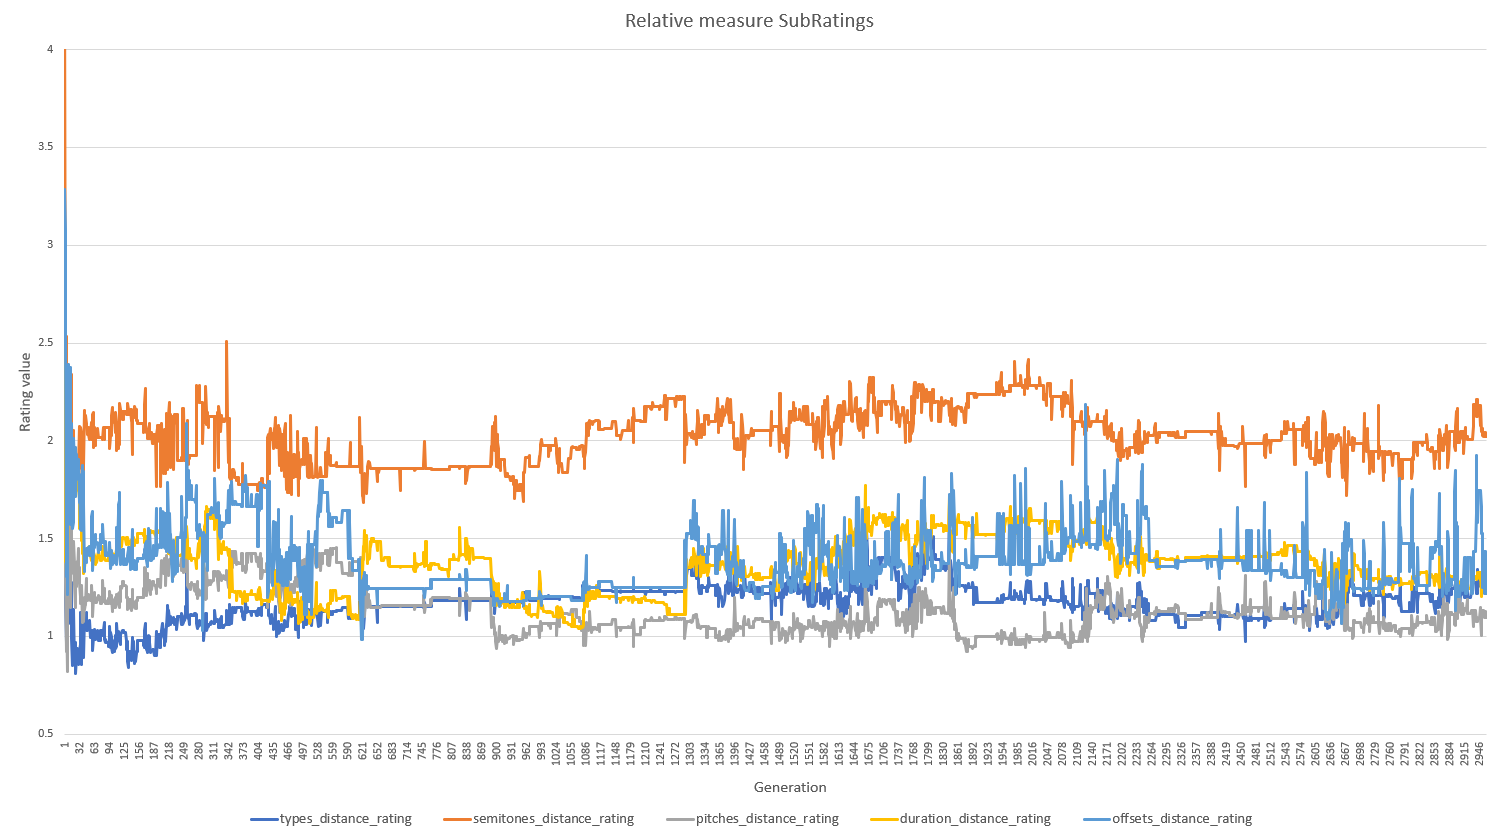
\includegraphics[width=1.2\textwidth]{Fotos/results/gf/rel_measures_rating_graph.png}
	\caption{Chart represents relative measure sub-raters over generations.}
	\label{fig:gf_relm}
\end{figure}

The absolute sub-raters can be split into two groups: those who get better and those who do not. If we leave out the initial drop-down that is always present on the start, we can see that the absolute rhythm, interval distribution distance and absolute type sub-ratings do not get better. It just moves around a fixed point. The other sub-ratings, however, have no problem lowering their value towards the bottom. All this is displayed on the chart on figure \ref{fig:gf_absolute}.


\begin{figure}[H]
	\advance\leftskip-1.5cm
	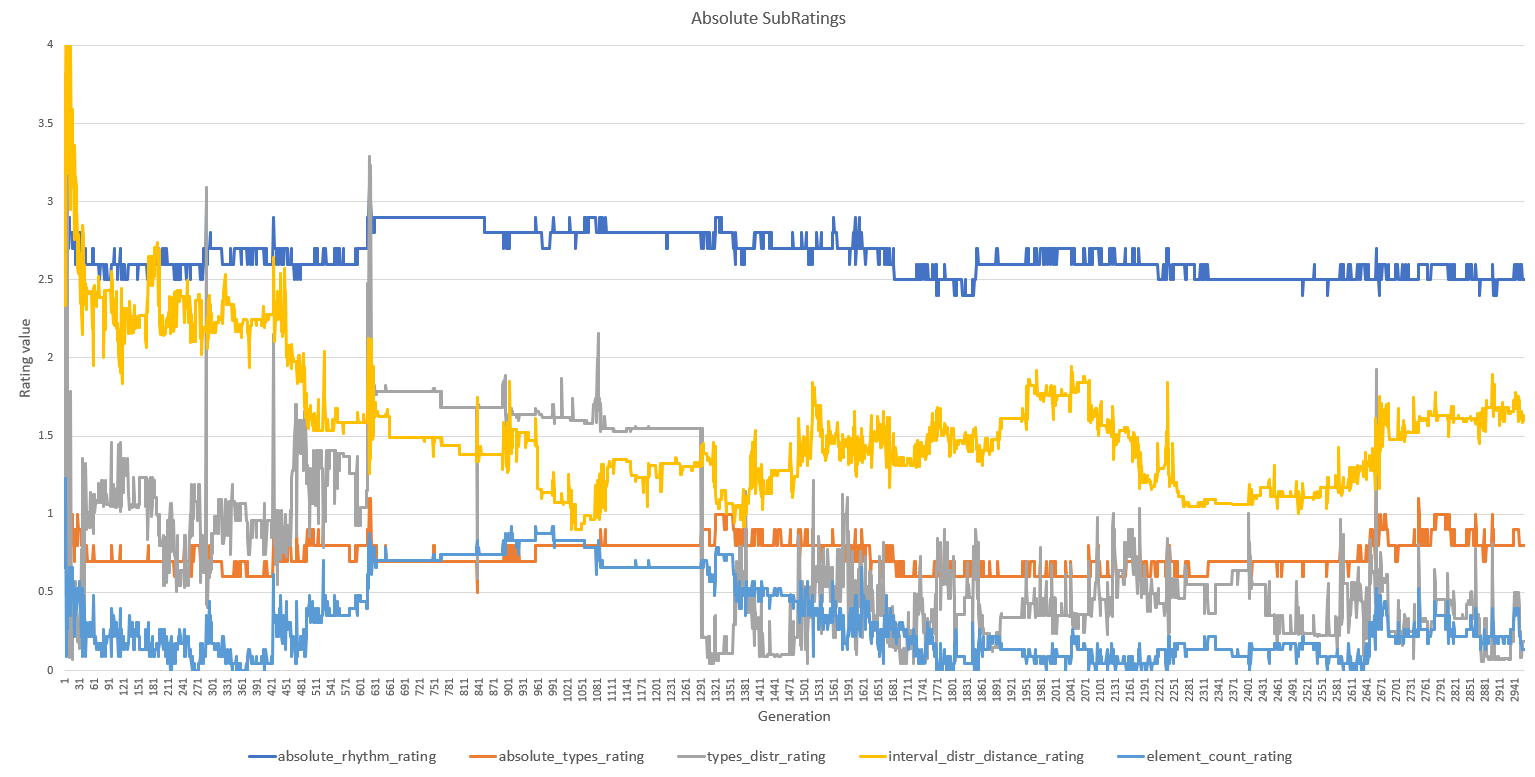
\includegraphics[width=1.2\textwidth]{Fotos/results/gf/absolute_rating_graph.png}
	\caption{Chart represents the absolute sub-raters over generations.}
	\label{fig:gf_absolute}
\end{figure}


Let us look closely into the last generations song and on the best-rated song in all of the generations, the song in generation 2454. On figure \ref{fig:strong_graph_last} and \ref{fig:strong_graph_best} we draw the charts of the strong measures of the latest song and the best song in that order.


\begin{figure}[H]
	\begin{center}
	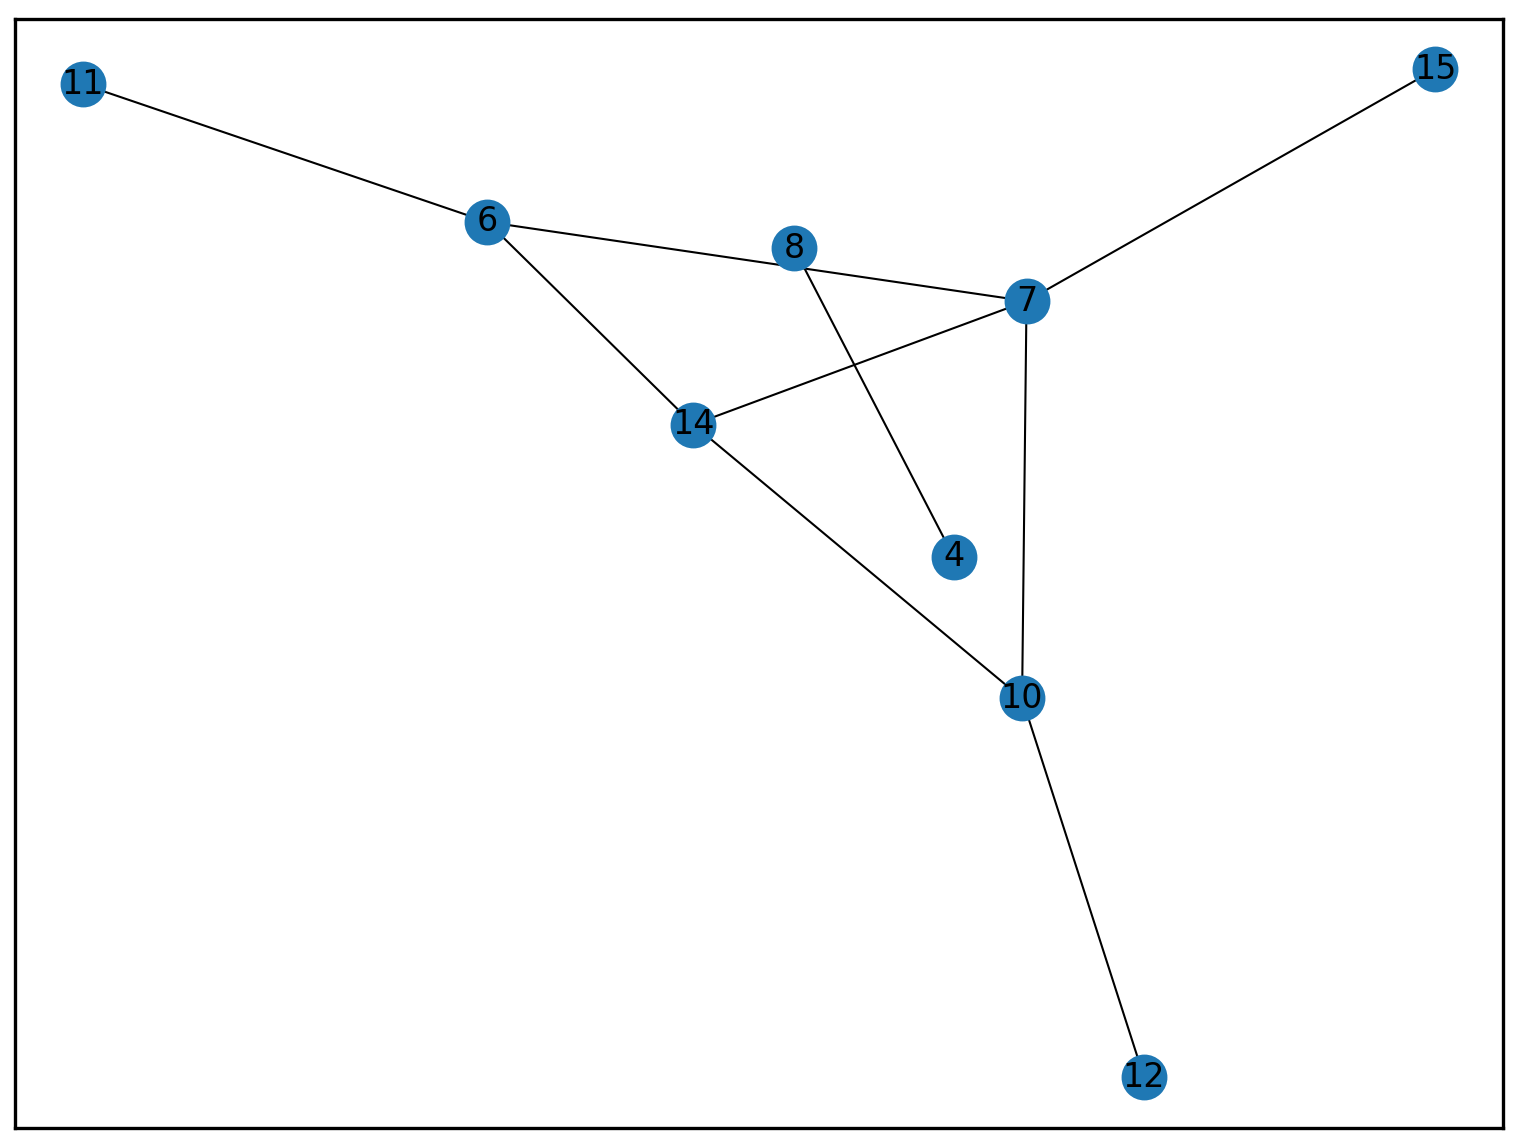
\includegraphics[width=0.8\textwidth]{Fotos/results/gf/strong_graph_last.png}
\end{center}
	\caption{Chart representing strong bindings between measures of generation 2960's song: 9 nodes, 9 bindings.}
	\label{fig:strong_graph_last}
\end{figure}


\begin{figure}[H]
	\begin{center}
	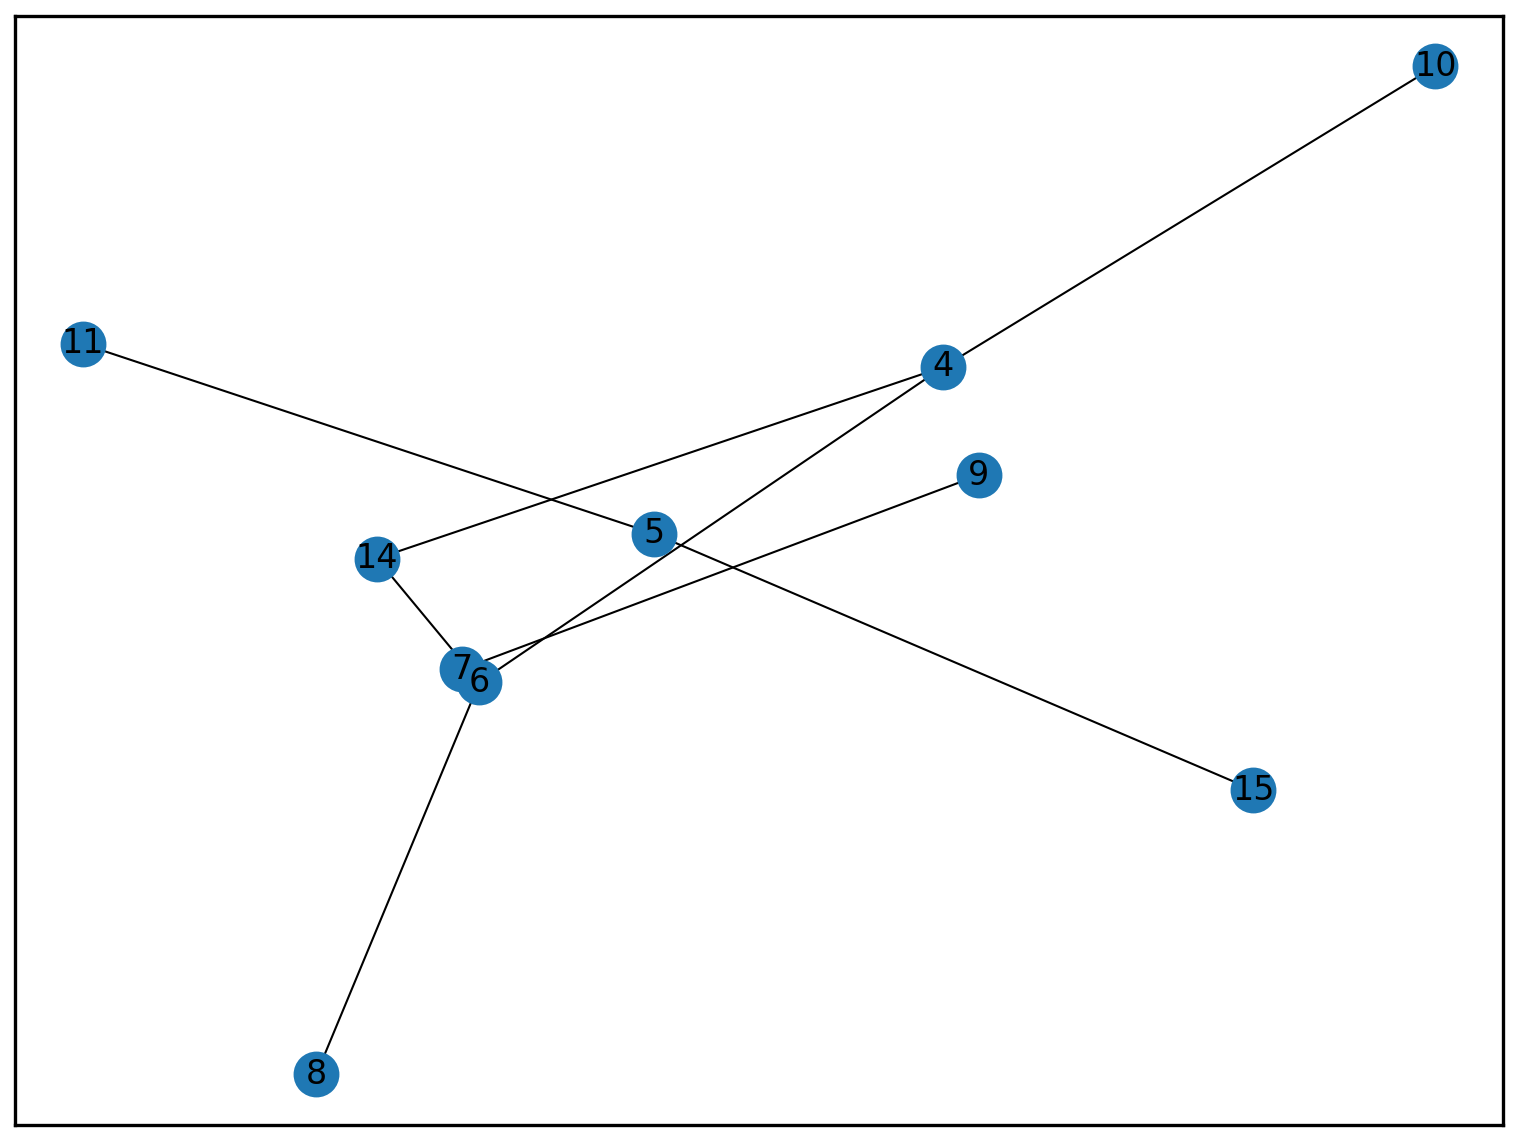
\includegraphics[width=0.8\textwidth]{Fotos/results/gf/strong_graph_best.png}
	\end{center}
	\caption{Chart representing strong bindings between measures of generation 2454's song: 10 nodes, 9 bindings.}
	\label{fig:strong_graph_best}
\end{figure}


These charts do not differ that much from each other. They have the exact same number of bindings, however, the best song has one node more meaning a stronger measure more which should be worse because the master got only 6 bindings. On listing \ref{code:last_song_scores} and \ref{code:best_song_scores} we have displayed the scores of both songs.

\begin{lstlisting}[language=Python,caption={Last gen song's ratings.},captionpos=b,label=code:last_song_scores]
total_rating: 13.71158427671084

scale_correctness_rating: 0.8059533386967015
zipfs_law_distance_pitches: 0.048321429478429545
zipfs_law_distance_intervals: 0.504584404235304

neighbour_pitch_rating: 0.0
melody_direction_rating: 0.0032455135547918568
direction_stability_rating: 0.0032455135547918568
unique_pitches_rating: 0.004558404558404561

bindings_rating: 0.31250000000000017
measures_rating: 0.0

types_distance_rating: 1.2331770314718207
semitones_distance_rating: 2.022577581521212
pitches_distance_rating: 1.0962565107329063
duration_distance_rating: 1.2384878914214006
offsets_distance_rating: 1.2206901412632365

absolute_rhythm_rating: 2.5
absolute_types_rating: 0.8
types_distr_rating: 0.18360655737704962
interval_distr_distance_rating: 1.602801011476367
element_count_rating: 0.13157894736842105
\end{lstlisting}


\begin{lstlisting}[language=Python,caption={Best gen song's ratings.},captionpos=b,label=code:best_song_scores]
total_rating: 12.586631765481918

scale_correctness_rating: 0.7575757575757576
zipfs_law_distance_pitches: 0.006453936769918456
zipfs_law_distance_intervals: 0.006456586132587705

neighbour_pitch_rating: 0.0
melody_direction_rating: 0.0037037037037036535
direction_stability_rating: 0.0037037037037036535
unique_pitches_rating: 0.00433941404090657

bindings_rating: 0.10416666666666664
measures_rating: 0.0

types_distance_rating: 1.093159810424484
semitones_distance_rating: 1.9874885117490217
pitches_distance_rating: 1.145892411313911
duration_distance_rating: 1.4105813969598486
offsets_distance_rating: 1.3345868956952605

absolute_rhythm_rating: 2.5
absolute_types_rating: 0.7000000000000001
types_distr_rating: 0.2371814092953529
interval_distr_distance_rating: 1.115902964959569
element_count_rating: 0.17543859649122806

\end{lstlisting}

If we compare both songs rating we can see where it exactly is where the best song does better. The biggest difference is the ratings based on the Intervals. The intervals Zipf's law distance from master rating and the interval distribution distance from the master rating contribute for the most part of the difference. The bindings rating has some impact that is worth noticing. This is because the distribution between the weak and normal type intervals also play a big role in this sub-rating. The relative measure based ratings from section \ref{sec:relratings} are slightly worse in the best song than the last song. 

\paragraph{Final thoughts}\mbox{}\\
When listening to both songs it is hard to decide which song has better results. We were not able to put the spirit of the Godfather theme song into the generations. We think this has to do with the absolute raters. They contribute to the recognizability of the master in the created songs. 
\\\\
When we analysed the charts on figure \ref{fig:gf_relm} and \ref{fig:gf_absolute} we noticed that not all the sub-raters get better. We clearly cannot satisfy every rating at the same time. It seems like these sub-raters are harder to satisfy with the current setup of mutations or they are generally just harder to get better without interfering with other sub-raters success.


\subsubsection{Beethoven Op.10 No.1 - 16 measures 9 parents}
We used the following songs for the initial population:
\begin{itemize}
\item Portal 2 - Cara Mia
\item rhcp - Californication 
\item Debussy - Clair de Lune
\item Chopin Mazurka, Op. 7 No. 1
\item Queen - Bohemian Rhapsody 
\item Godfather theme song
\end{itemize}

This song has little to no strong bindings, although you can hear some patterns, there is almost no absolute repetition.
\\\\
We have lowered the number of songs selected for mutation from 70\% to 50\%. The probability for a mutation is still 20\%. We played with some weights: we increased the absolute sub-rater's weights by nearly doubling them, mainly because of the unimportance of the repetition. We would like to concentrate on the commonality between the master and the population. We got 9 parents and 4531 generations.
\\\\
As always, let us start with a chart representing the total rating over the generations. On figure \ref{fig:beethoven_1} a chart with the total rating over generations has been illustrated.

\begin{figure}[H]
	\advance\leftskip-1.5cm
	\includegraphics[width=1.2\textwidth]{Fotos/results/beethoven/total_rating_graph.png}
	\caption{Graph for total rating with: master song the Beethoven Op.10 No.1, 16 measures, 9 children, very low measure mutation rates, 4531 generations.}
	\label{fig:beethoven_1}
\end{figure}

We can clearly see that after a while, progress gets rarer. There are still fluctuations, this is because of the mutations having a big impact on the children. There where an upstroke occurs, we always find that the generation before that had at least 7 out of the 9 parents selected for mutation. This means that we need to lower the probability or need more parents. However, we cannot guarantee fast results with more than 9 parents. \\\\
Let us examine the best-rated song. This song can be found in generation 3479.

\begin{lstlisting}[language=Python,caption={Best gen song's ratings.},captionpos=b,label=code:beethoven_best_song_scores]
total_rating: 17.375831003462814

scale_correctness_rating: 0.40652680652680656
zipfs_law_distance_pitches: 0.17059384950989798
zipfs_law_distance_intervals: 0.035466943947383145

neighbour_pitch_rating: 0.0
melody_direction_rating: 0.02022792022792025
direction_stability_rating: 0.1279202279202279
unique_pitches_rating: 0.0004940711462450564

bindings_rating: 0.062499999999999986
measures_rating: 0.46875

types_distance_rating: 1.0328232229473218
semitones_distance_rating: 1.6175795730068843
pitches_distance_rating: 0.9578696140205788
duration_distance_rating: 1.0420890693702636
offsets_distance_rating: 2.077841941339121

absolute_rhythm_rating: 5.2
absolute_types_rating: 2.2
types_distr_rating: 0.0618729096989965
interval_distr_distance_rating: 1.8932748538011692
element_count_rating: 0.0
\end{lstlisting}

If we look at the absolute values on listing \ref{code:beethoven_best_song_scores} of the song and of the songs in all generations, we noticed just like we did before that they do not get tend to lower themselves. When we compare the song to the master, we can see similarities.

\begin{figure}[H]
	\advance\leftskip-1.5cm
	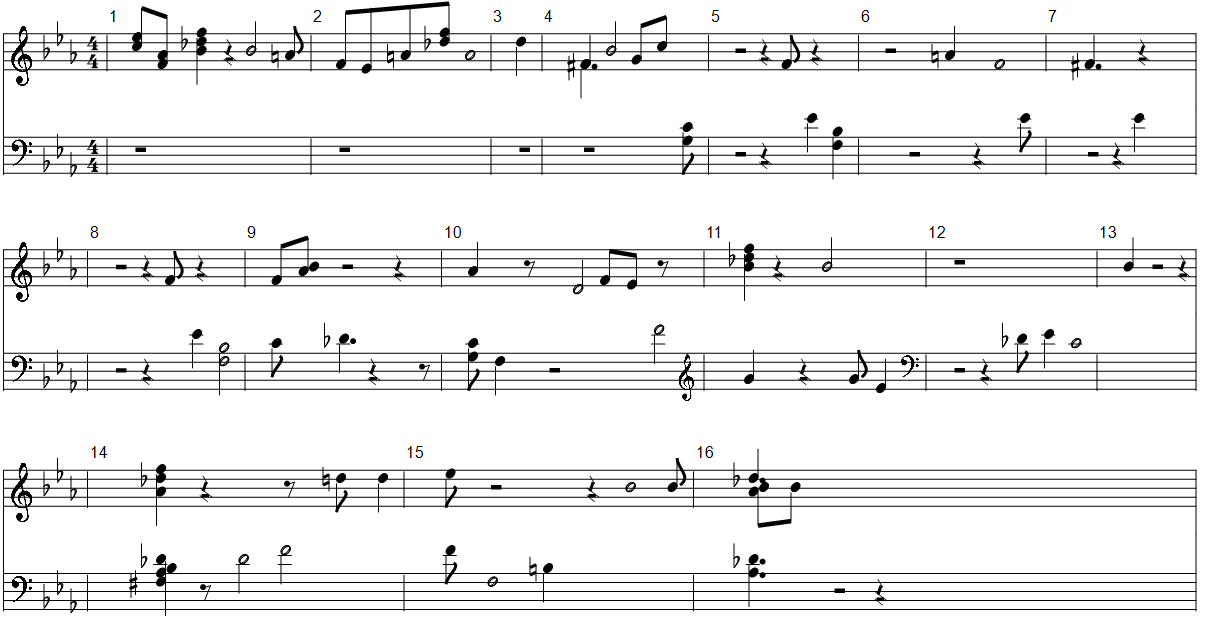
\includegraphics[width=1.2\textwidth]{Fotos/results/beethoven/best.png}
	\caption{The Best song overall out of generation of 3479 generations.}
	\label{fig:beethoven_best}
\end{figure}

\begin{figure}[H]
	\advance\leftskip-1.5cm
	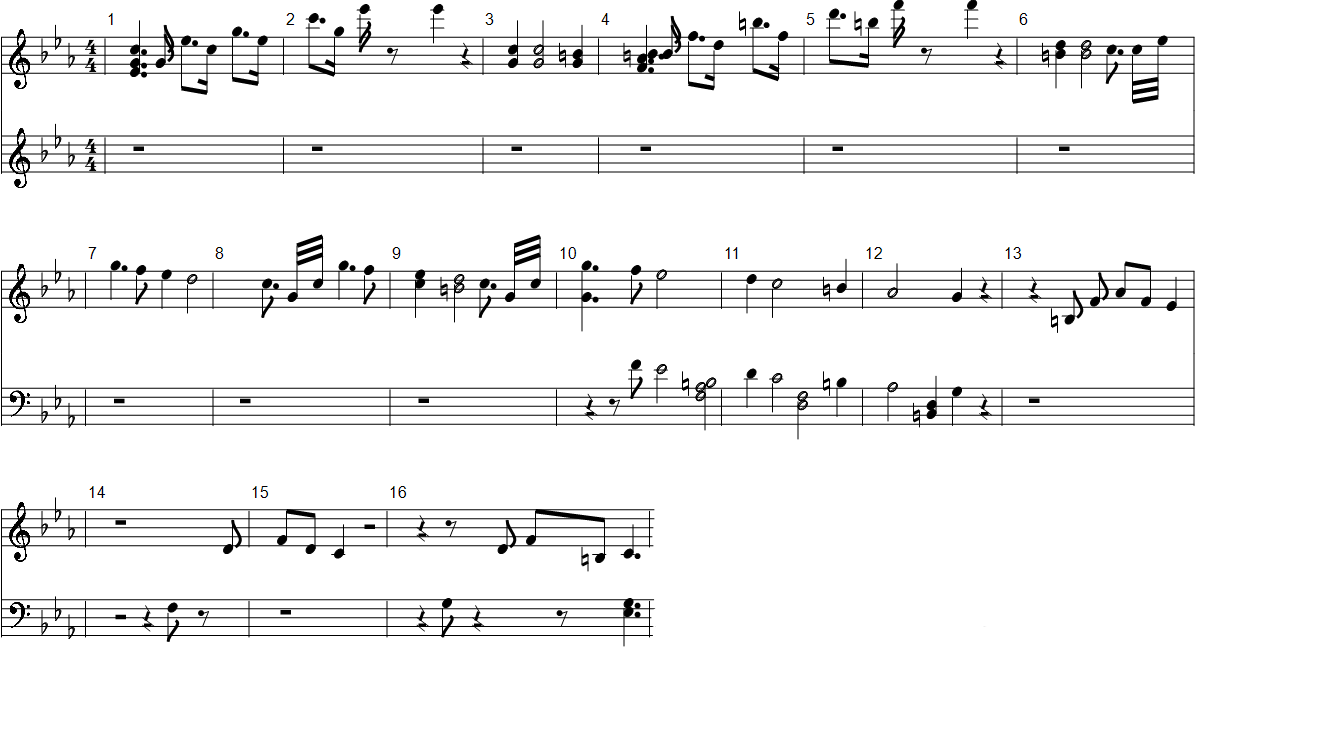
\includegraphics[width=1.2\textwidth]{Fotos/results/beethoven/beethoven_measures.png}
	\caption{The master song: Beethoven Op.10 No.1.}
	\label{fig:beethoven_master}
\end{figure}

Even though the songs do not look like each other, we can detect commonalties. On figure \ref{fig:beethoven_best} and \ref{fig:beethoven_master} we illustrated both songs for comparison. We can see that some patterns from the master are recognizable in the best song. The Godfather goes upwards during the first two measures, this is noticeable in our best-generated song, especially in the 2nd measure. There where there are a few elements, our best song tends to have fewer elements. The opposite tends to be also true, more elements in some parts in the master means more elements in our best song around that exact part.

\paragraph{Final thoughts}\mbox{}\\
This was a clear result of the mutations not being able to proceed towards the master's style. Even though there are recognizable items, it is not enough. There is a still lack of some concepts in our process.

\section{Conclusion}
We compared three big executions were we got useful results. We have concentrated on the measures and their behaviour and relationship with one and another. This made it easier to create repetitive patterns as we concluded in our first execution with a highly repetitive master.

\subsection{Theory based vs. sample based}
We have not been able to get strong results from the theory-based strategies. We moved towards the sample-based strategy because they provided a path that we could follow: the path to the master. Because we based a reasonable amount of our sub-raters on the master, we found it more interesting to analyze the sample-based strategy rather than a theory-based.
\\\\
The sample-based strategy provided interesting results compared to the theory-based were the songs were just a mix of the initial songs with some mutations. We did not know what we're trying to achieve, at least not as clearly as we knew when we used a master.

\subsection{Genetic algorithm, Mutations, Planning and Ratings}
We can say that a genetic algorithm is not ideal when time and resources are potential issues. We cannot simply do random stuff and hope that we can catch the best out of these random actions. Although we planned mutation like the selection of wrong intervals and worst rated measures, it was not enough. We believe that a more planned approach would have faster for achieving good results. Still, planning does come with its dangers. If we plan to change things in an algorithmic manner we may exclude other possible solutions. Solutions we may only be able to achieve by randomized actions, we can call this some sort of creativity. This creativity can be responsible to achieve good results in different ways. We can use this creativity to catch strategies that result in good results and use these in another implementation where we add them to the planning list. So we would have two implementations, one where we discover strategies, the other where we implement all these strategies discovered in the previous implementation and try to achieve good results as fast as possible.
\\\\
If we would have used more planned actions, the mutations would have happened based on where the songs rated the lowest. Trying to fix those first and trying to focus on that. 
\\\\
Mutations are the key to transformation in any direction, good or bad. We need to try to prevent the bad from happening. We do not necessarily have to try to put the mutations in good order, just preventing the bad could be the deal-breaker. In other words, we need to be able to make mistakes in a song with mutation, but not inherit those mutations into the next generation or at least take the pre-mutated song with them as well.
\\\\
We saw that some ratings did not get better but even got worse. This has mainly to do with the weights. By defining some weights heavier than others, we introduced the concept of importance between sub-raters. This proves that there is a deeper understanding necessary for the correct distribution of these weights. More information about what actually makes a song that what it is can be useful for this. For example, when analyzing a master song, we can try to look where the master song is scoring better than its other components and try to focus the weights on that part. So if we found out that the repetition level is high and we know that achieving this level is hard, we can put a higher value on this weight because we know that this sub-rating is a deal-breaker. We did this manually in our first run by increasing the measure weights.
\\\\
We surely know that we were not able to cover all concepts out of the music domain that are out there. An increase in the number of sub-raters would probably create better results. The same for mutations, there could have been more different types of mutations that had a direct impact on every sub-rater there is.
\\\\
Fuzzy matching is not known to be the best matching algorithm when it comes to musical pitches and intervals. We know for example that $A3$ and $C4$ are closer to each other than $A3$ and $E4$, but the fuzzy matching algorithm does not. This could be improved by implementing a matching system specifically for this use.

\subsection{Selection}
We noticed in the analysis of the results that the total rating of the next generation can be worse than the previous one. An implementation where we always kept the best song ever achieved in the generation would have prevented this from ever happening. This way we could have kept the progress that has been made so far.

\subsection{Crossover}
When it comes to the crossover process, it could have been done in a more advanced and correct way. The known problem where it is possible to have a gap in a certain part of the song could have been eliminated by simply choosing one or the other song's sound at that point. So the gap between the offsets 3.5 and 4.0 on figure \ref{fig:cross_7} could have been prevented by just simply making a choice between song A and B and filling it with their corresponding parts.

\subsection{music21}
It is said that the music21 library has both been helpful and problematic. Even though it was the best library we could find, it came with its flaws that we had to solve in our own way. The least we could do is to prevent them from happening. A home-made implementation where we could easily swap notes measures and so on would have been useful. We could better have used the library in combination with our own implementation.


\subsection{Music and more}
A deeper understanding of music is necessary when the goal is to achieve better results, which we currently noticed that we did not possess enough. There is still uncharted domain that we have not been able to explore, analyze and implement. These are the so-called dimensions that we excluded from our implementation to lower its complexity. One of them would have been the introduction of patterns in volume, this would have added a whole new dimension to our project. The addition of multiple layers played by different instruments can also be a big deal.
\\\\
Nevertheless, it has come clear that composing music with a genetic algorithm can be effective when we got the necessary tools. We believe that both time and a complete implementation of rules and concepts from music will successfully compose music towards an already existing master song. If we can analyze a song completely with every detail, dimension, pattern and so on, it should be possible to create another song similar to it.




\newpage
\begin{thebibliography}{9}


\bibitem{copyright} 
Copyright infringement
\\\url{https://en.wikipedia.org/wiki/Copyright_infringement}

\bibitem{magma} 
Adil H. Khan. 
\textit{"Artificial Intelligence approaches to music composition"}. 
Highland Heights, Kentucky, October 14th, 2013


\bibitem{genjam} 
John A. Biles 
\textit{"GenJam: A Genetic Algorithm for Generating Jazz Solos"}. 
In ICMC Proceedings 1994, The Computer Music Association, 1994.
Rochester Institute of Technology

\bibitem{genetic} 
Dragan MATIĆ
\textit{"A genetic Algorithm for composing music"}. 
Faculty of Natural Sciences University of Banjaluka, Bosnia and Herzegovina, April 2010



\bibitem{genmusictheory} 
Michael Towsey, Andrew Brown, Susan Wright and Joachim Diederich
\textit{"Towards Melodic Extension Using Genetic Algorithms"}. 
Queensland University of Technology, 2001, Kelvin Grove, QLD 4059, Australia



\bibitem{genmusicbach} 
Viktor Anderling, Olle Andreasson, Christoffer Olsson, Sean Pavlov, Christian Svensson, Johannes Wikner
\textit{"Generation of music through genetic algorithms"}. 
Chalmers University of Technology
University of Gothenburg
Department of Computer Science and Engineering
Gothenburg, Sweden, June 2014



\bibitem{piano_midi} 
Classical Piano Midi Page 
\\\url{http://www.piano-midi.de}

\bibitem{BitMidi} 
BitMidi
\\\url{https://bitmidi.com}

\bibitem{jmusic} 
jMusic: Computer music composition in Java.
\\\url{http://explodingart.com/jmusic/}

\bibitem{music21} 
Music21: a toolkit for computer-aided musicology
\\\url{https://web.mit.edu/music21/}

\bibitem{jfugue} 
JFugue: Music Programming for Java and JVM Languages 
\\\url{http://www.jfugue.org/}


\bibitem{Zipfslaw} 
Zipf's law
\\\url{https://en.wikipedia.org/wiki/Zipf's_law}

\bibitem{FuzzyWuzzy} 
FuzzyWuzzy library
\\\url{https://github.com/seatgeek/fuzzywuzzy}

\bibitem{Levenshtein_distance} 
Levenshtein distance
\\\url{https://en.wikipedia.org/wiki/Levenshtein_distance}



\bibitem{Zipfslaw_paper} 
Bill Manaris, Juan Romero, Penousal Machado, Dwight Krehbiel, Timothy Hirzel,Walter Pharr, and Robert B. Davis
\textit{"Zipf's Law, Music Classification, and Aesthetics"}. 
Computer Science Department, College of Charleston
March 13, 2006


\bibitem{wasserstein_python} 
scipy.stats.wasserstein distance
\\\url{https://docs.scipy.org/doc/scipy/reference/generated/scipy.stats.wasserstein_distance.html}


\bibitem{wasserstein_paper} 
Tom Quareme,P rof. dr. Philippe Bekaert, dr. Nick Michiels, dr. Jeroen Put
\textit{"Towards Polygonal Mesh Generation With Generative Adversarial Networks"}. 
Faculty of Sciences: Computer Science, Hasselt University, Belgium




\end{thebibliography}




\end{document}





























